\documentclass{beamer}
\usetheme{}
\usecolortheme{dolphin}           
\useinnertheme{circles}
\setbeamertemplate{itemize items}[default]
\setbeamertemplate{enumerate items}[default]
\usepackage[T1]{fontenc}
\usepackage[utf8]{inputenc}
\usepackage{lmodern}
\usepackage{amsmath}
\usepackage{booktabs} 
\usepackage{graphicx}        
\usepackage{array}
\usepackage{color}
\usepackage{textcomp}
\usepackage{epstopdf}
\makeatletter
\def\zapcolorreset{\let\reset@color\relax\ignorespaces}
\def\colorrows#1{\noalign{\aftergroup\zapcolorreset#1}\ignorespaces}
\makeatother
\graphicspath{{/home/swl/Dropbox/ucd/international_trade/tex/}} 
\setbeamertemplate{navigation symbols}{}


%--------------------------------------
%%%% DETAILS TITLE PAGE %%%%
%--------------------------------------
\title{Gravity model}
\author{School of Economics, University College Dublin}
\date{Autumn 2017}
\begin{document}
%--------------------------------------
%%%% TITLE SLIDE %%%%
%--------------------------------------
\begin{frame}
\titlepage  
\end{frame}

%--------------------------------------
\begin{frame}
  Does Ireland export more to Belgium or to China?
\end{frame}
%--------------------------------------

%--------------------------------------
\begin{frame}
  \begin{figure}\centering
    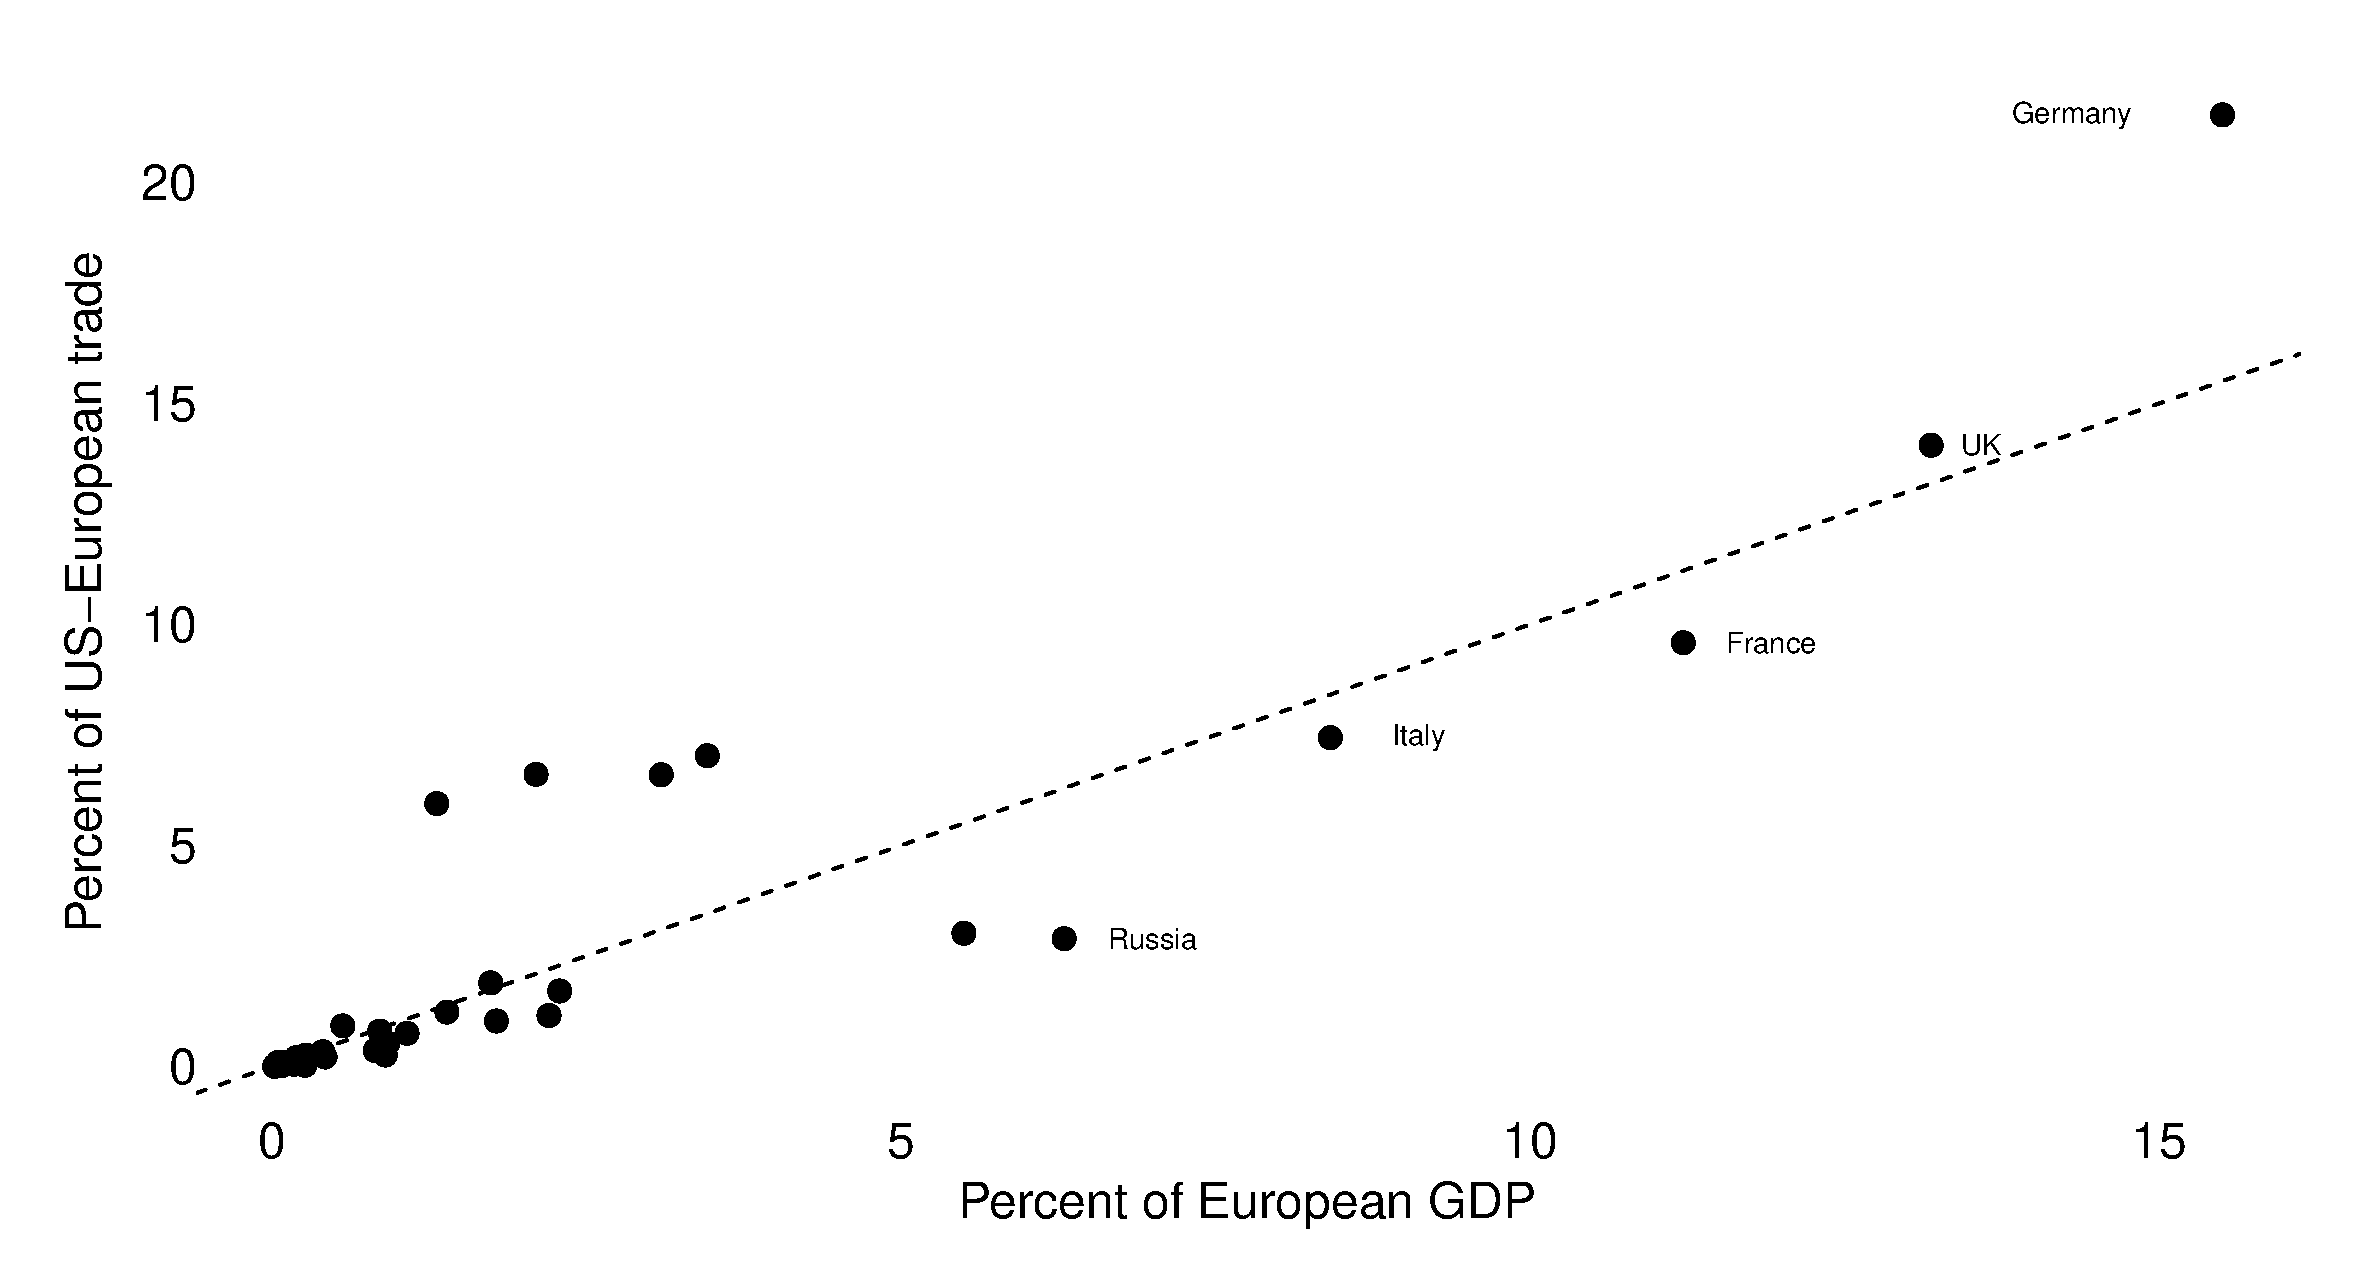
\includegraphics[scale=.25]{us_gravity}
  \end{figure}
\end{frame}
%--------------------------------------

%--------------------------------------
\begin{frame}
  For the US, the three largest European trading partners are also the three largest European economies.
  \medskip  
  \begin{enumerate}
    \item Why does U.S. trade more with these countries rather than other European economies?
    \item What explains almost linear relationship between GDP and trade flows?
  \end{enumerate}
\end{frame}
%--------------------------------------

%--------------------------------------
\begin{frame}
  \textbf{Size matters:}
  Jan Tinbergen found out in 1962 that trade volume is directly related to the size of the economy 
  \medskip
    \begin{enumerate}
      \item Larger economies produce more and thus have to sell more in export market
      \item Larger economies generate more income and are thus able to buy more imports
    \end{enumerate}
\end{frame}
%--------------------------------------

%--------------------------------------
\begin{frame}
\begin{figure}
  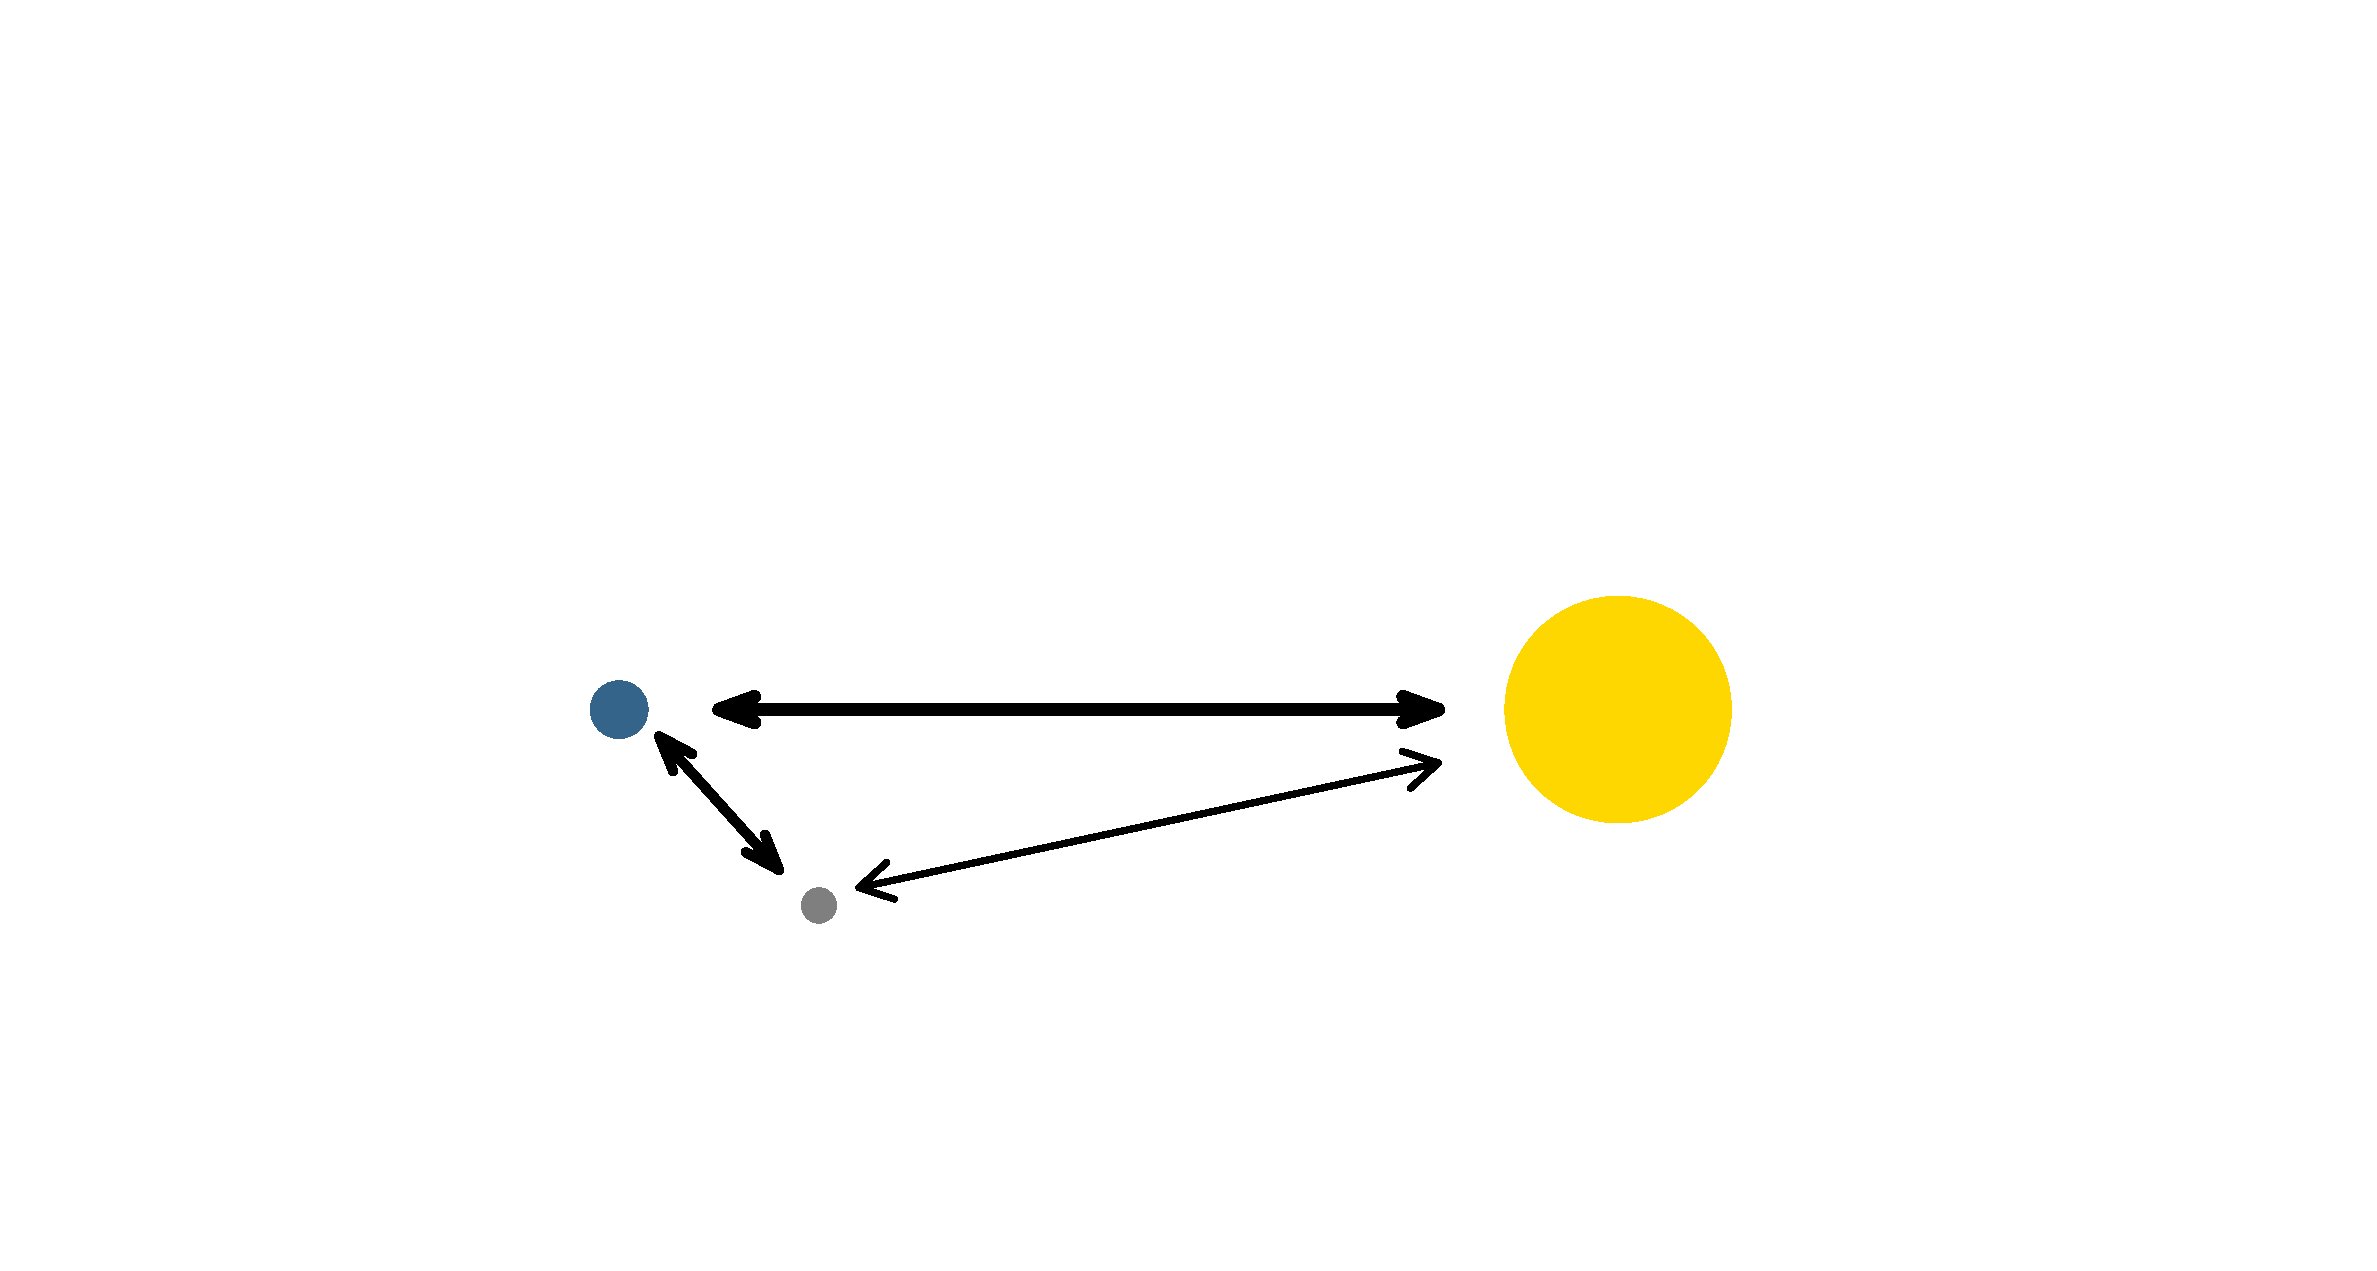
\includegraphics[scale=.25]{gravity2}
\end{figure}
  \begin{align*}
    F_{ij} = G \frac{M_1 M_2}{r^2}
  \end{align*}
$M_i$ is the mass of the object\\
$r$ is the distance between the objects\\
$G$ is a gravitational constant \footnote{$6.67*10^{-11} N(m/kg)^2$}
\end{frame}
%--------------------------------------

%--------------------------------------
\begin{frame}
  Trade between countries is similar to gravitational force between objects
  \begin{itemize}
    \item Objects with large mass, or those that are close together, have greater gravitational pull between them
  \end{itemize}
  \medskip
  This implies that there will be more trade between countries if
    \begin{enumerate}
      \item Countries have large economies
      \item Countries are close to each other
    \end{enumerate}    
\end{frame}
%--------------------------------------

%--------------------------------------
\begin{frame}
  In 2015 Ireland exported 
  \begin{itemize}
    \item 12\% of total to Belgium
    \item 3\% of total to China
  \end{itemize}
\end{frame}
%--------------------------------------

%--------------------------------------
\begin{frame}
  \begin{align*}
    T_{ij}=\alpha \frac{M_i^{\beta} M_j^{\gamma}}{D_{ij}^{\theta}}
  \end{align*}
$T_{ij}$ is trade flow from country $i$ to $j$\\
$M_i$ and $M_j$ are economic size of the two countries\\
$D_{ij}$ is the distance between the two countries
\end{frame}
%--------------------------------------

%--------------------------------------
\begin{frame}
  \begin{align*}
    T_{ij}\propto M_i^{\beta} M_j^{\gamma}
  \end{align*}
\begin{enumerate}
  \item Exports rise proportionally with economic size of destination country
  \item Imports increase in proportion to origin's country economic size
\end{enumerate}

  The model is short-hand for supply and demand forces
\begin{itemize}
  \item For origin country $i$
  \begin{itemize}
    \item $M_i$ represents total supply of $i$
    \item $M_j$ represents total demand of $j$
  \end{itemize}
\end{itemize}
\end{frame}
%--------------------------------------

%--------------------------------------
\begin{frame}
  \begin{align*}
    T_{ij} \propto \frac{1}{D_{ij}^{\theta}}
  \end{align*}

\begin{enumerate}
  \item $T_{ij}$ is decreasing in distance
\end{enumerate}
Distance basically acts as a tax, imposing trade costs, which results in lower equilibrium trade flows.
\end{frame}
%--------------------------------------

%--------------------------------------
\begin{frame}{UK exports in 2015}
\framesubtitle{source: Office for National Statistics}
  \begin{figure}
    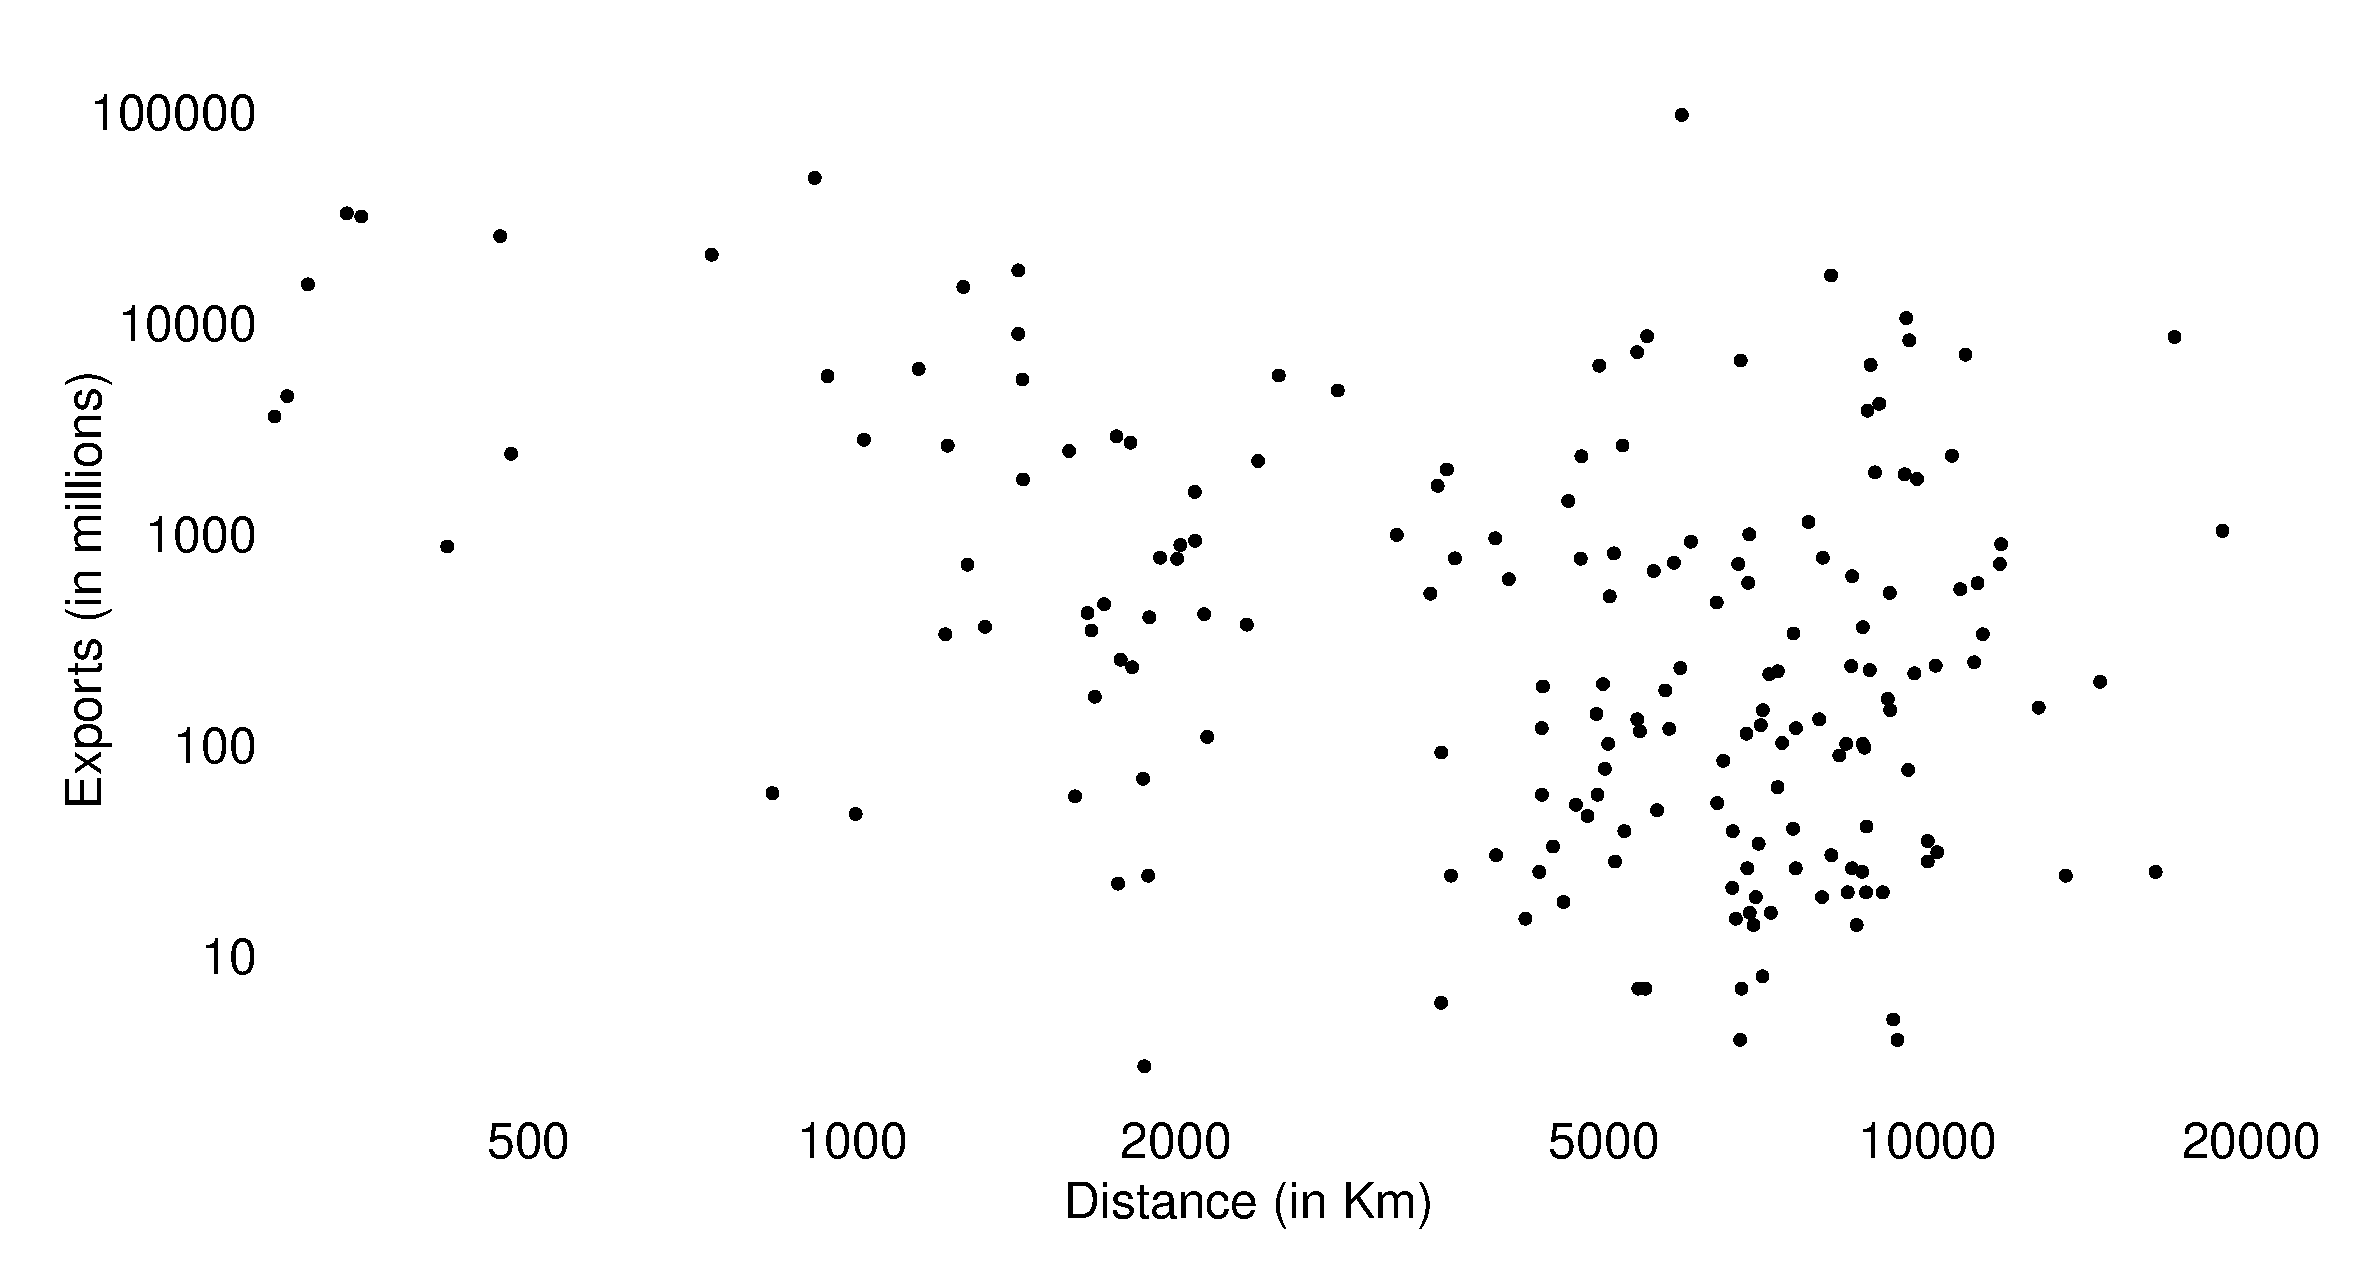
\includegraphics[scale=.25]{uk_gravity}
  \end{figure}  
\end{frame}
%--------------------------------------

%--------------------------------------
\begin{frame}
  In its simplest form only size and distance are important for trade. 
  \medskip
  Also note that 
  \begin{enumerate}
    \item Everything enters multiplicatively, including distance
    \item No 3rd country effects, except through GDP changes
  \end{enumerate}
  \medskip
  Despite being a very simple model, the gravity model has produced some of the most robust findings in economic research.
\end{frame}
%--------------------------------------

%--------------------------------------
\begin{frame}
  Log-linearisation:
  \begin{align*}
    ln(ab) &= ln(a)+ln(b)\\ 
    ln \left(\frac{a}{b} \right) &= ln(a) - ln(b)\\
    ln(a^b) &= b \cdot ln(a)
  \end{align*}
\end{frame}
%--------------------------------------


%--------------------------------------
\begin{frame}
  We can estimate the gravity model using OLS using log-linearisation, so    
    \begin{align*}
    T_{ij}=\alpha \frac{M_i^{\beta} M_j^{\gamma}}{D_{ij}^{\theta}}
  \end{align*}
  becomes
  \begin{align*}
    ln \; T_{ij}= ln\; \alpha + \beta \; ln \; M_i + \gamma \; ln \; M_j - \theta \; ln \; D_{ij}
  \end{align*}
  We can generalise this and add an error term to produce regression model
  \begin{align*}
    ln\; T_{ij} = \theta \; ln\; D_{ij} + \beta \; ln\; M_i + \gamma\; ln\; M_j + \epsilon_{ij}
  \end{align*} 
  \medskip
  Except distance coefficient $\theta<0$ and $\beta=\gamma=1$  
\end{frame}
%--------------------------------------

%--------------------------------------
\begin{frame}
  Economic mass $M$ often measured by GDP
  \begin{itemize}
    \item Estimated coefficients close to 1; range from 0.7 to 1.1
  \end{itemize}
  \medskip
  Including $M_i,M_j$ as regressors leads to inflated $R^2$ values
    \begin{enumerate}
      \item Large economies will trade more in absolute terms
      \item Trade is part of GDP so simultaneity between $T_{ij},M_i,M_j$
    \end{enumerate}  
\end{frame}
%--------------------------------------

%--------------------------------------
\begin{frame}{Imports and Exports Japan-EU, 2006}
\framesubtitle{Head and Mayer, 2013}
  \begin{figure}\centering
    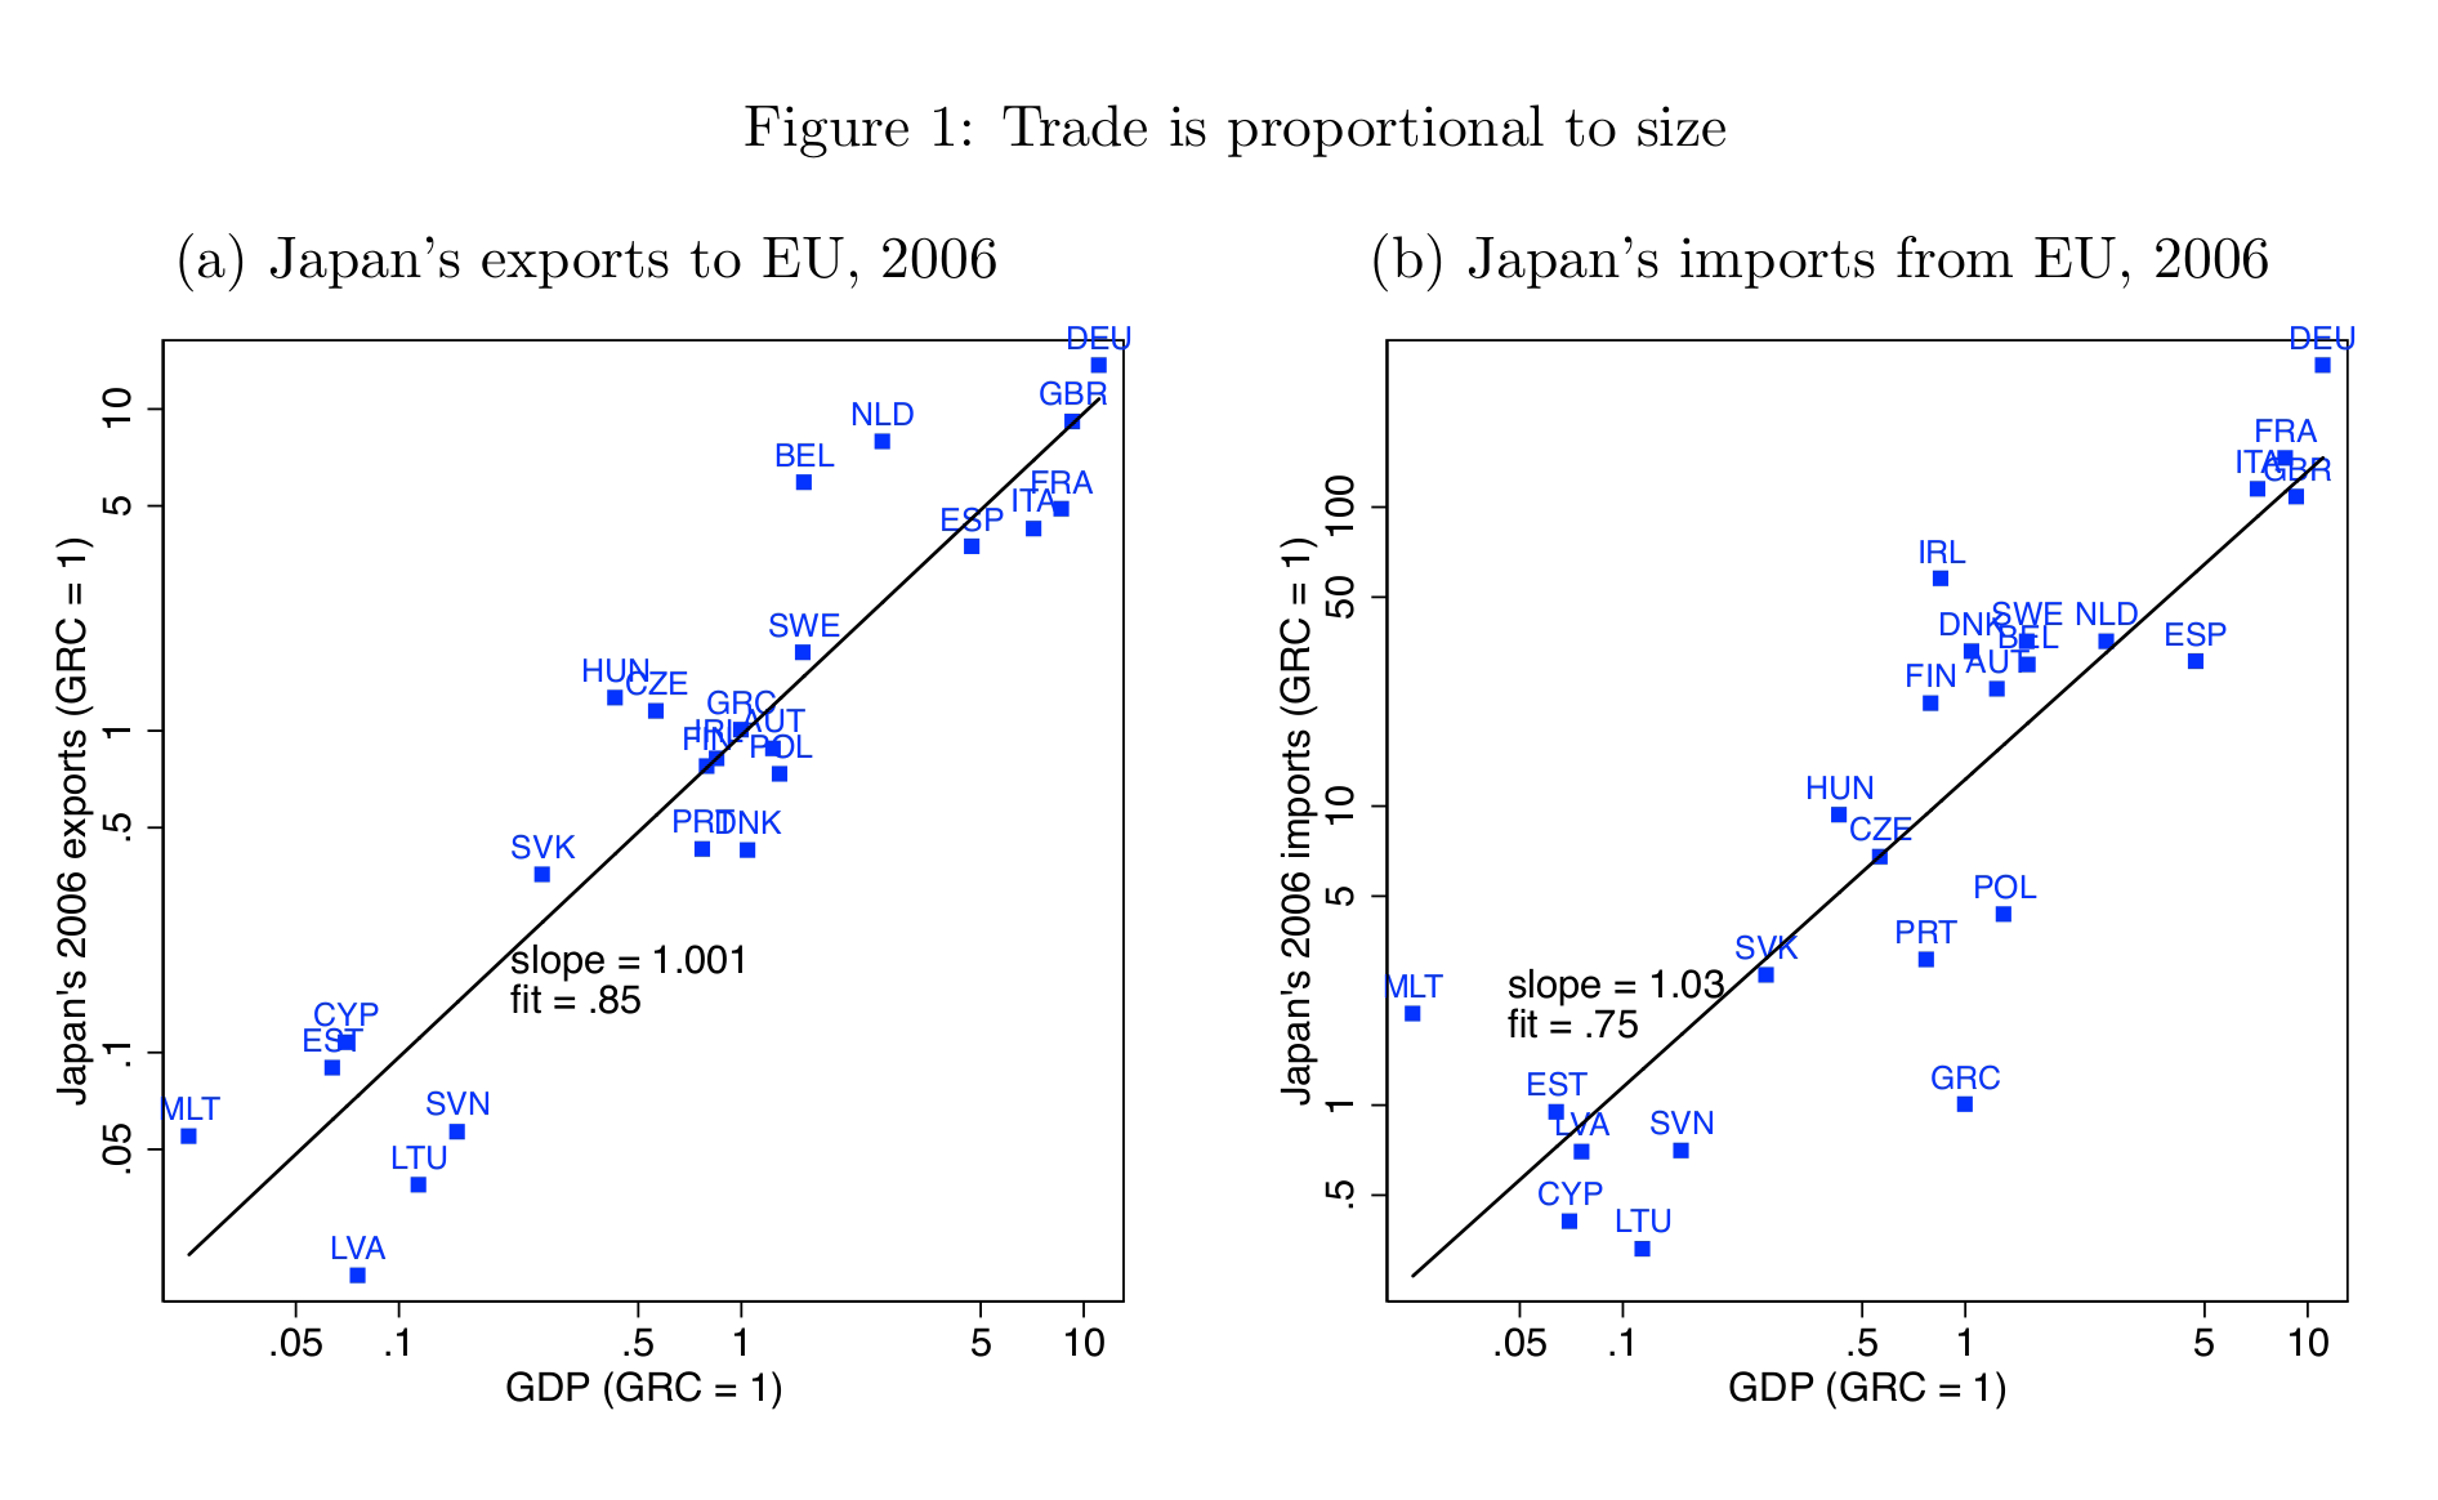
\includegraphics[scale=.1]{head_mayer}
  \end{figure}  
\end{frame}
%--------------------------------------

%--------------------------------------
\begin{frame}
  $D$ often based on great circle distance
    \begin{itemize}
      \item Length of straight line across surface of a sphere
      \item Underestimates the true distance
    \end{itemize}
    \medskip
  1\% increase in distance associated with 0.7-1\% loss in trade volume, so doubling the distance could reduce trade by half. 
  \begin{itemize}
    \item Effect could be attributed to substitution elasticity between goods from different countries
  \end{itemize}
  \medskip
  The distance associated trade costs seem rather large.
\end{frame}
%--------------------------------------

%--------------------------------------
\begin{frame}
  The gravity model has been estimated over a thousand times, so no harm in doing it again.
  \begin{itemize}
    \item Using a square gravity dataset for all country-pairs in the world between 1948-2006
  \end{itemize} 
   Estimate
  \begin{align*}
    Trade \;flow_{ij} = \beta_1 GDP_i + \beta_2 GDP_j + \beta_3 Distance_{ij}
  \end{align*}
  \begin{itemize}
    \item Subset data to 2006 and drop zero flows
    \item Use natural logs
  \end{itemize}
\end{frame}
%--------------------------------------


%--------------------------------------
\begin{frame}
  \begin{figure}\centering
    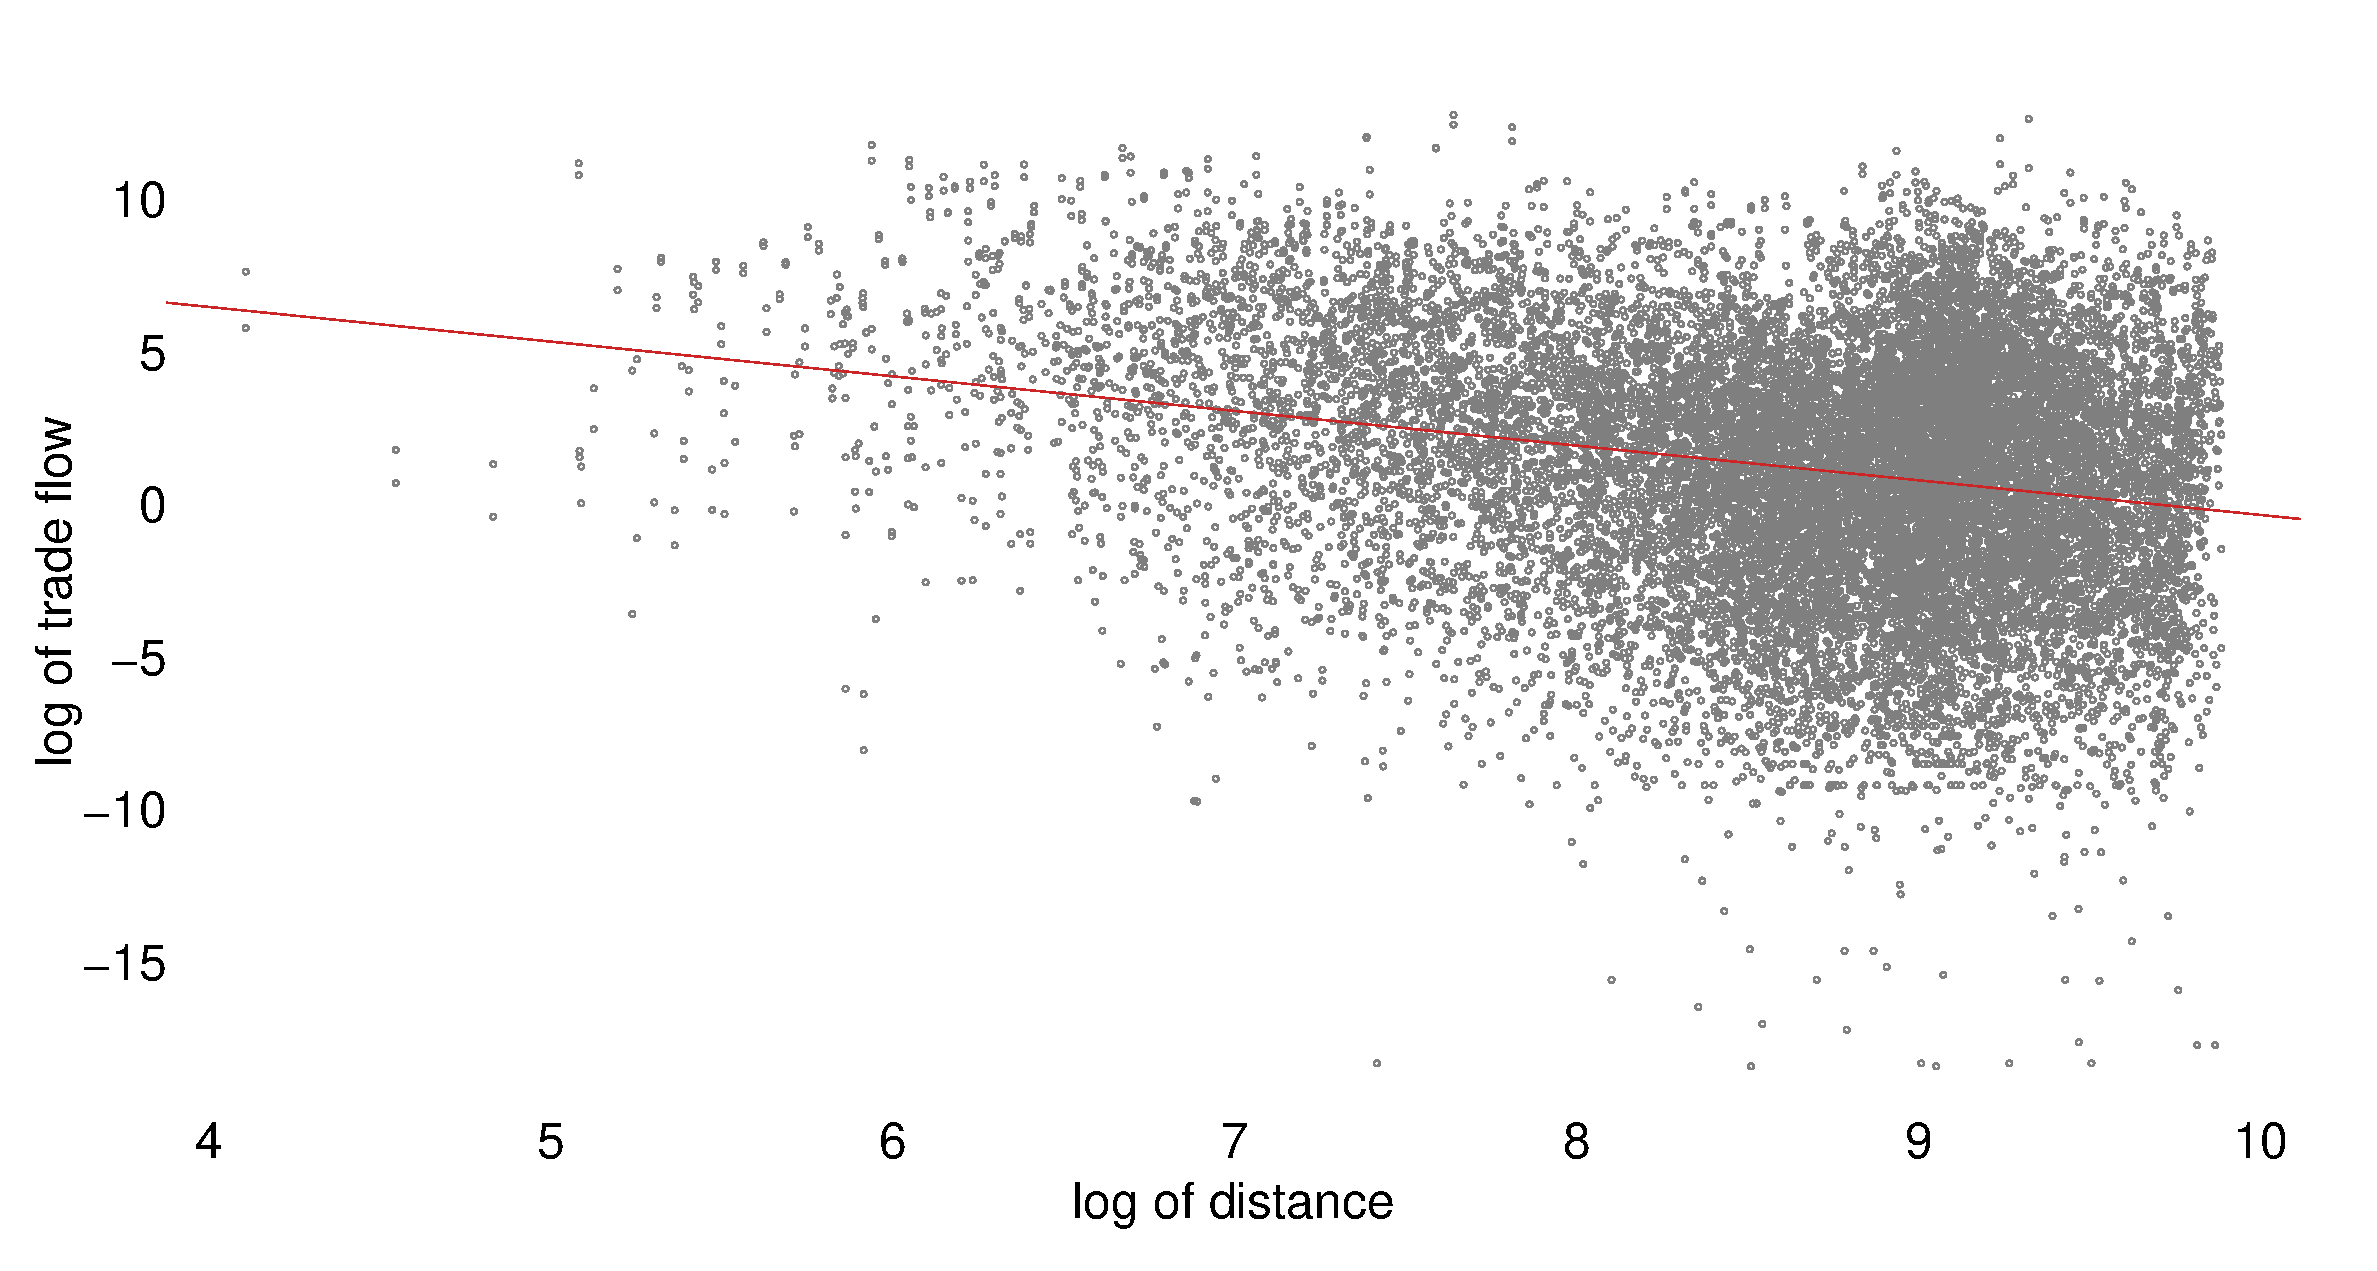
\includegraphics[scale=.3]{gravity_estimated}
  \end{figure}
\end{frame}
%--------------------------------------

%--------------------------------------
\begin{frame}
  For 2006 the regression shows that $\hat{\theta}=-1.52, \; (\pm 0.02) $\footnote{$R^2=0.63, N=17,088$}
  \begin{itemize}
    \item i.e. a 1\% increase in distance is associated with a 1.52\% decline in trade flows
  \end{itemize}
  Can repeat this process looking at the other years to see how the estimated effect changes over time.  
\end{frame}
%--------------------------------------

%--------------------------------------
\begin{frame}
  \begin{figure}
    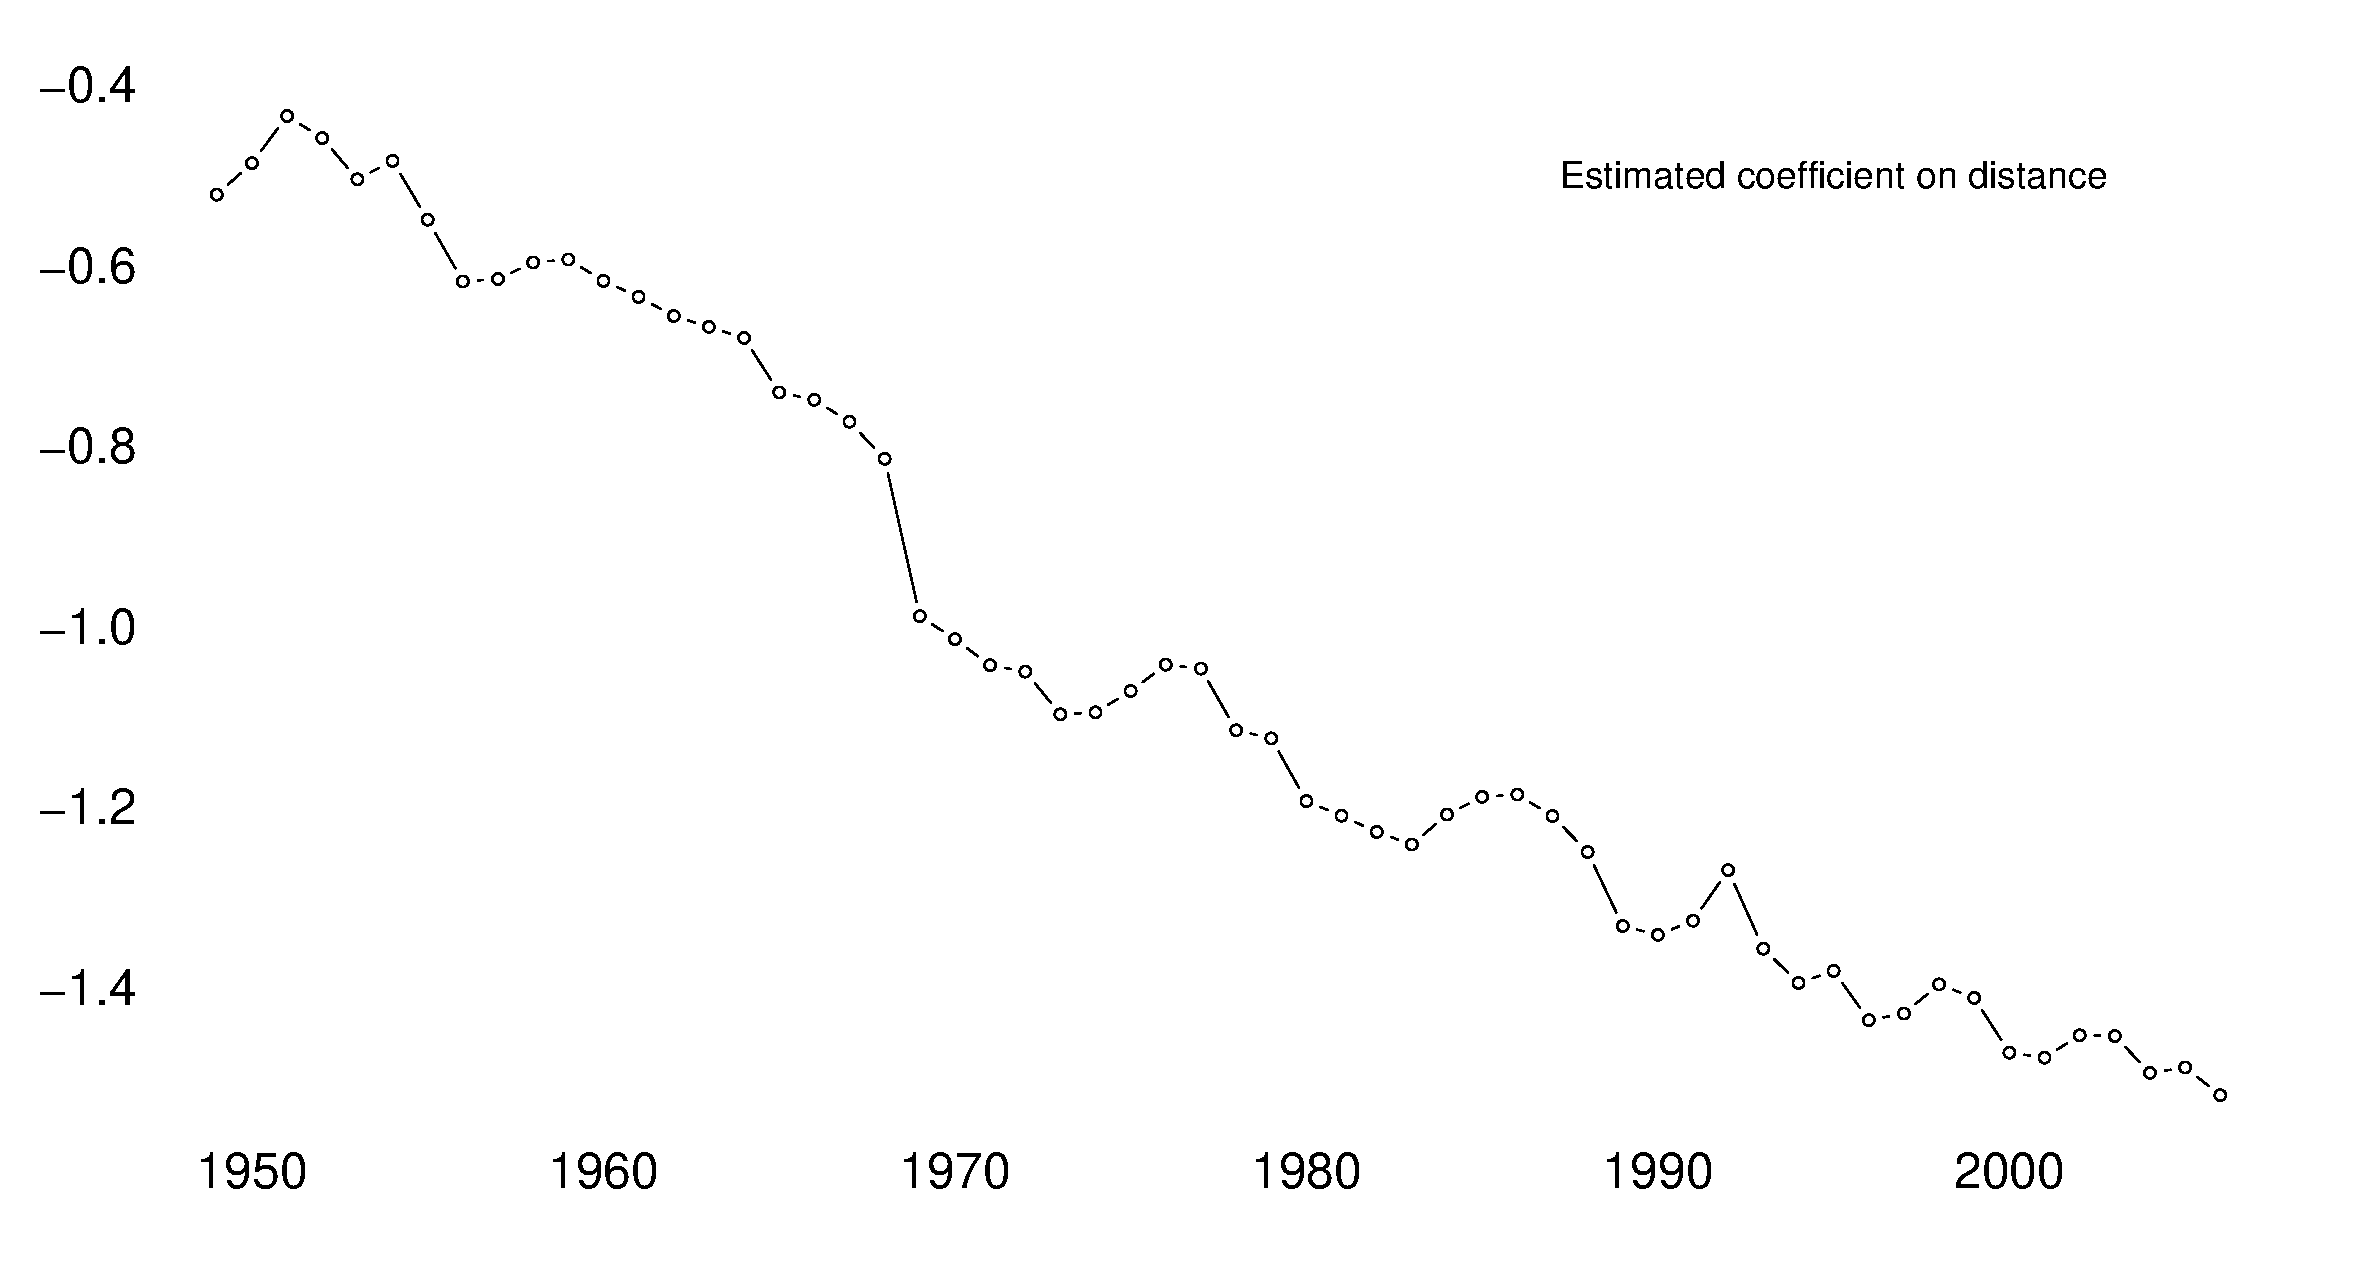
\includegraphics[scale=.3]{coef_distance}
  \end{figure}
\end{frame}
%--------------------------------------

%--------------------------------------
\begin{frame}{Disdier \& Head (2008)}
  \begin{figure}
    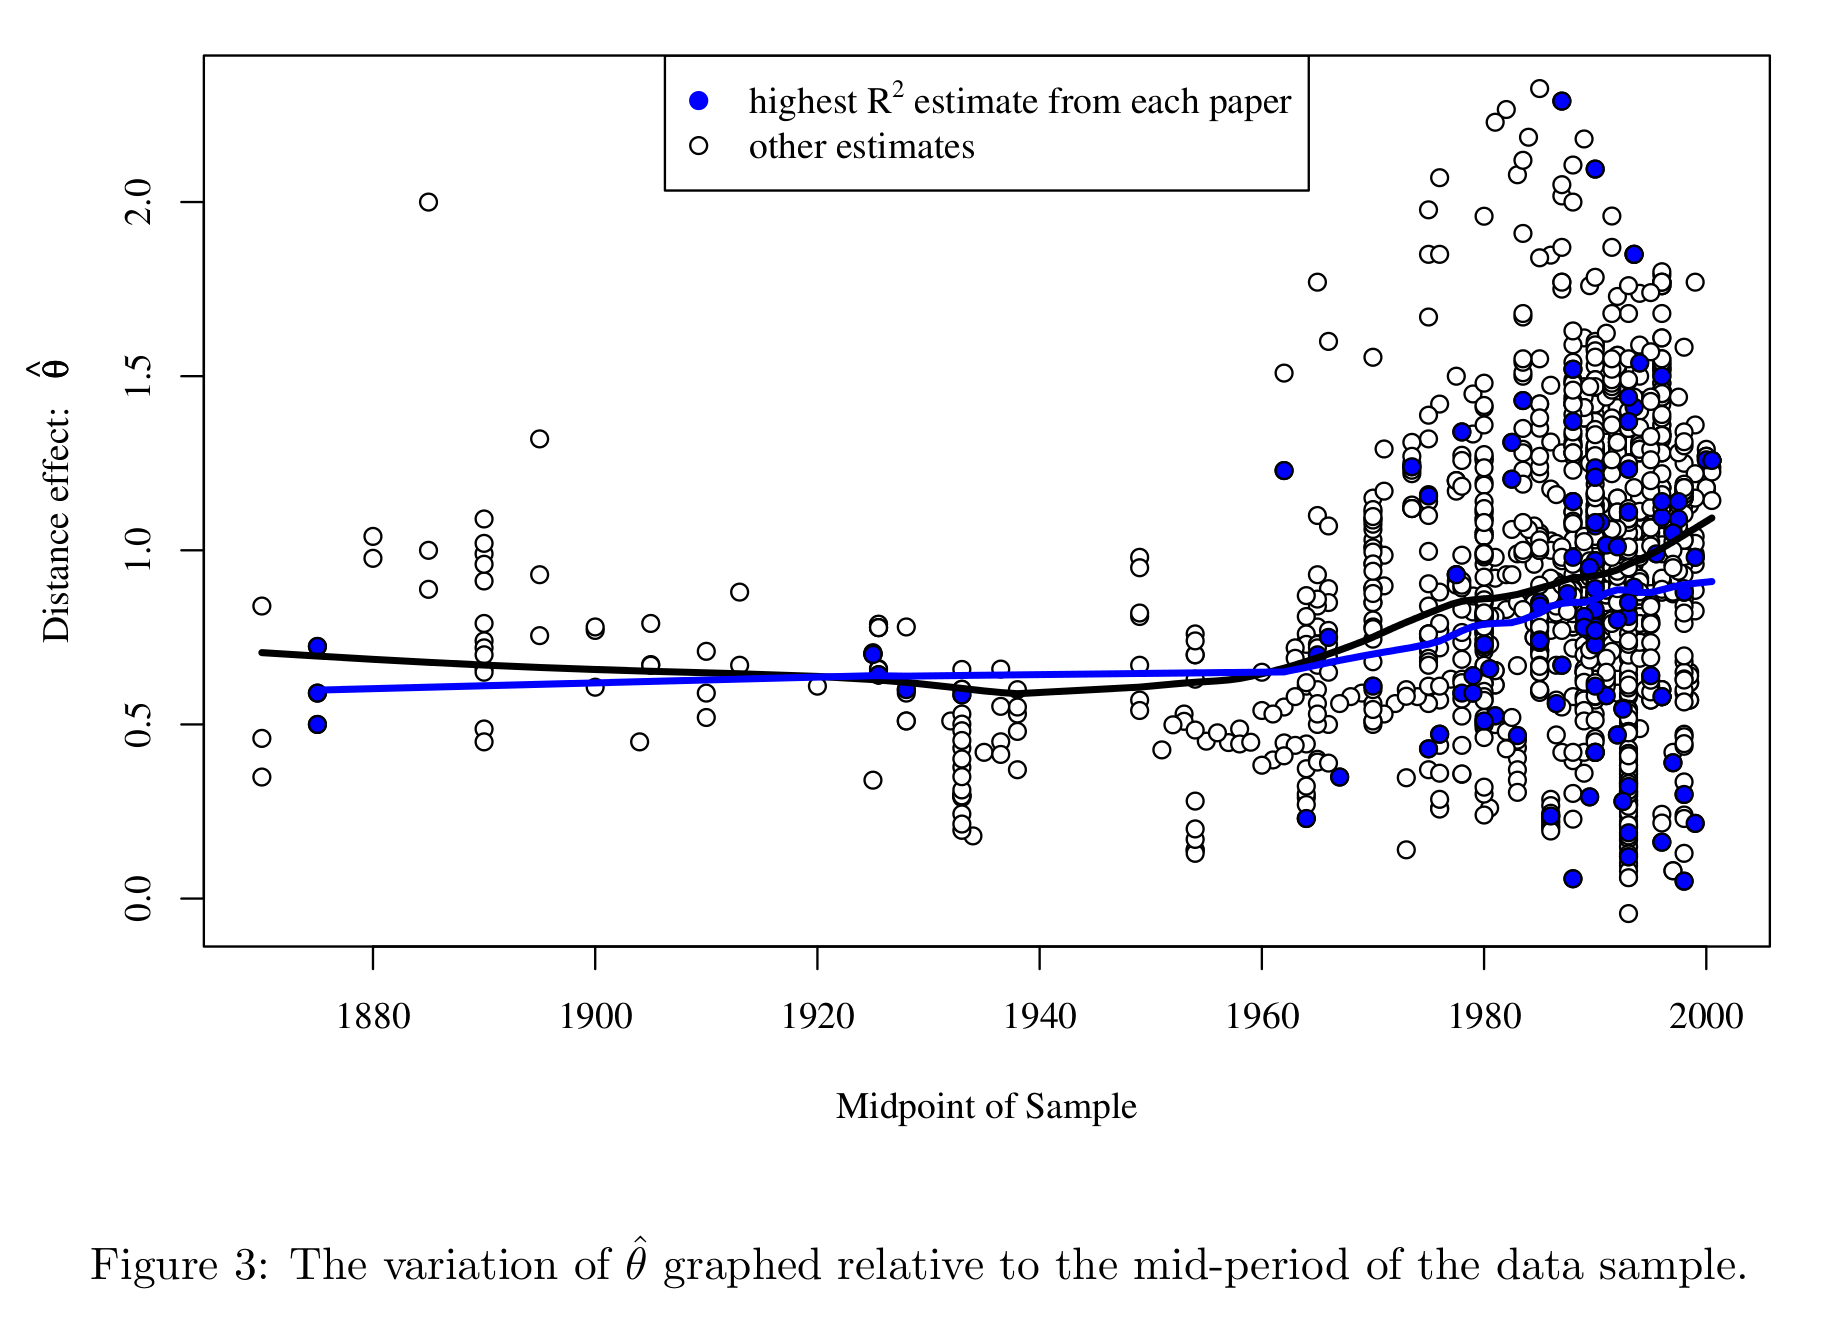
\includegraphics[scale=.7]{disdier_head}
  \end{figure}
\end{frame}
%--------------------------------------

%--------------------------------------
\begin{frame}
  Effect of distance increases over time.
  Some possible explanations for this include
  \medskip
  \begin{itemize}
    \item Omitted variable bias 
    \item Trade costs have increased (unlikely)
    \item Regional trade agreements divert trade 
    \item People have become more responsive to price differences
  \end{itemize}
\end{frame}
%--------------------------------------

%--------------------------------------
\begin{frame}{Recall this guy}
  \begin{figure}\centering
    
\includegraphics[scale=.1]{lego}
  \end{figure}
\end{frame}
%--------------------------------------

%--------------------------------------
\begin{frame}
  Gravity increasing possibly due to vertical disintegration
  \begin{itemize}
    \item When the production of a product crosses multiple national borders
  \end{itemize}
  If a product is shipped multiple time during production, it could lead to being counted in trade data more than once
\end{frame}

%--------------------------------------
\begin{frame}
  Economists have offered six explanations for why distance matters so much.
  \medskip
  \begin{enumerate}
    \item Proxy for transport costs
    \begin{itemize}
      \item e.g. freights charges, insurance
    \end{itemize}
    \item Indication of time elapsed during shipment
    \begin{itemize}
      \item Damage or loss of shipment 
      \item Decomposition/spoiling of organic goods
      \item Loss of market
    \end{itemize}
  \end{enumerate}  
\end{frame}
%--------------------------------------

%--------------------------------------
\begin{frame}
  \begin{enumerate}
    \item[3.] Synchronisation costs
    \begin{itemize}
      \item Sourcing inputs from nearby lowers synchronisation costs
    \end{itemize}
    \item[4.] Communication costs
    \begin{itemize}
      \item Exchange of information via less formal methods
    \end{itemize}
    \item [5.] Transaction costs
    \begin{itemize}
      \item Search for trade opportunities
      \item Establishment of trust between trade partners
    \end{itemize}
    \item[6.] Cultural distance
  \end{enumerate}  
\end{frame}
%--------------------------------------

%--------------------------------------
\begin{frame}{Percentage of firms that export}
\framesubtitle{Croezet and Koenig, 2010}
  \begin{figure}\centering
    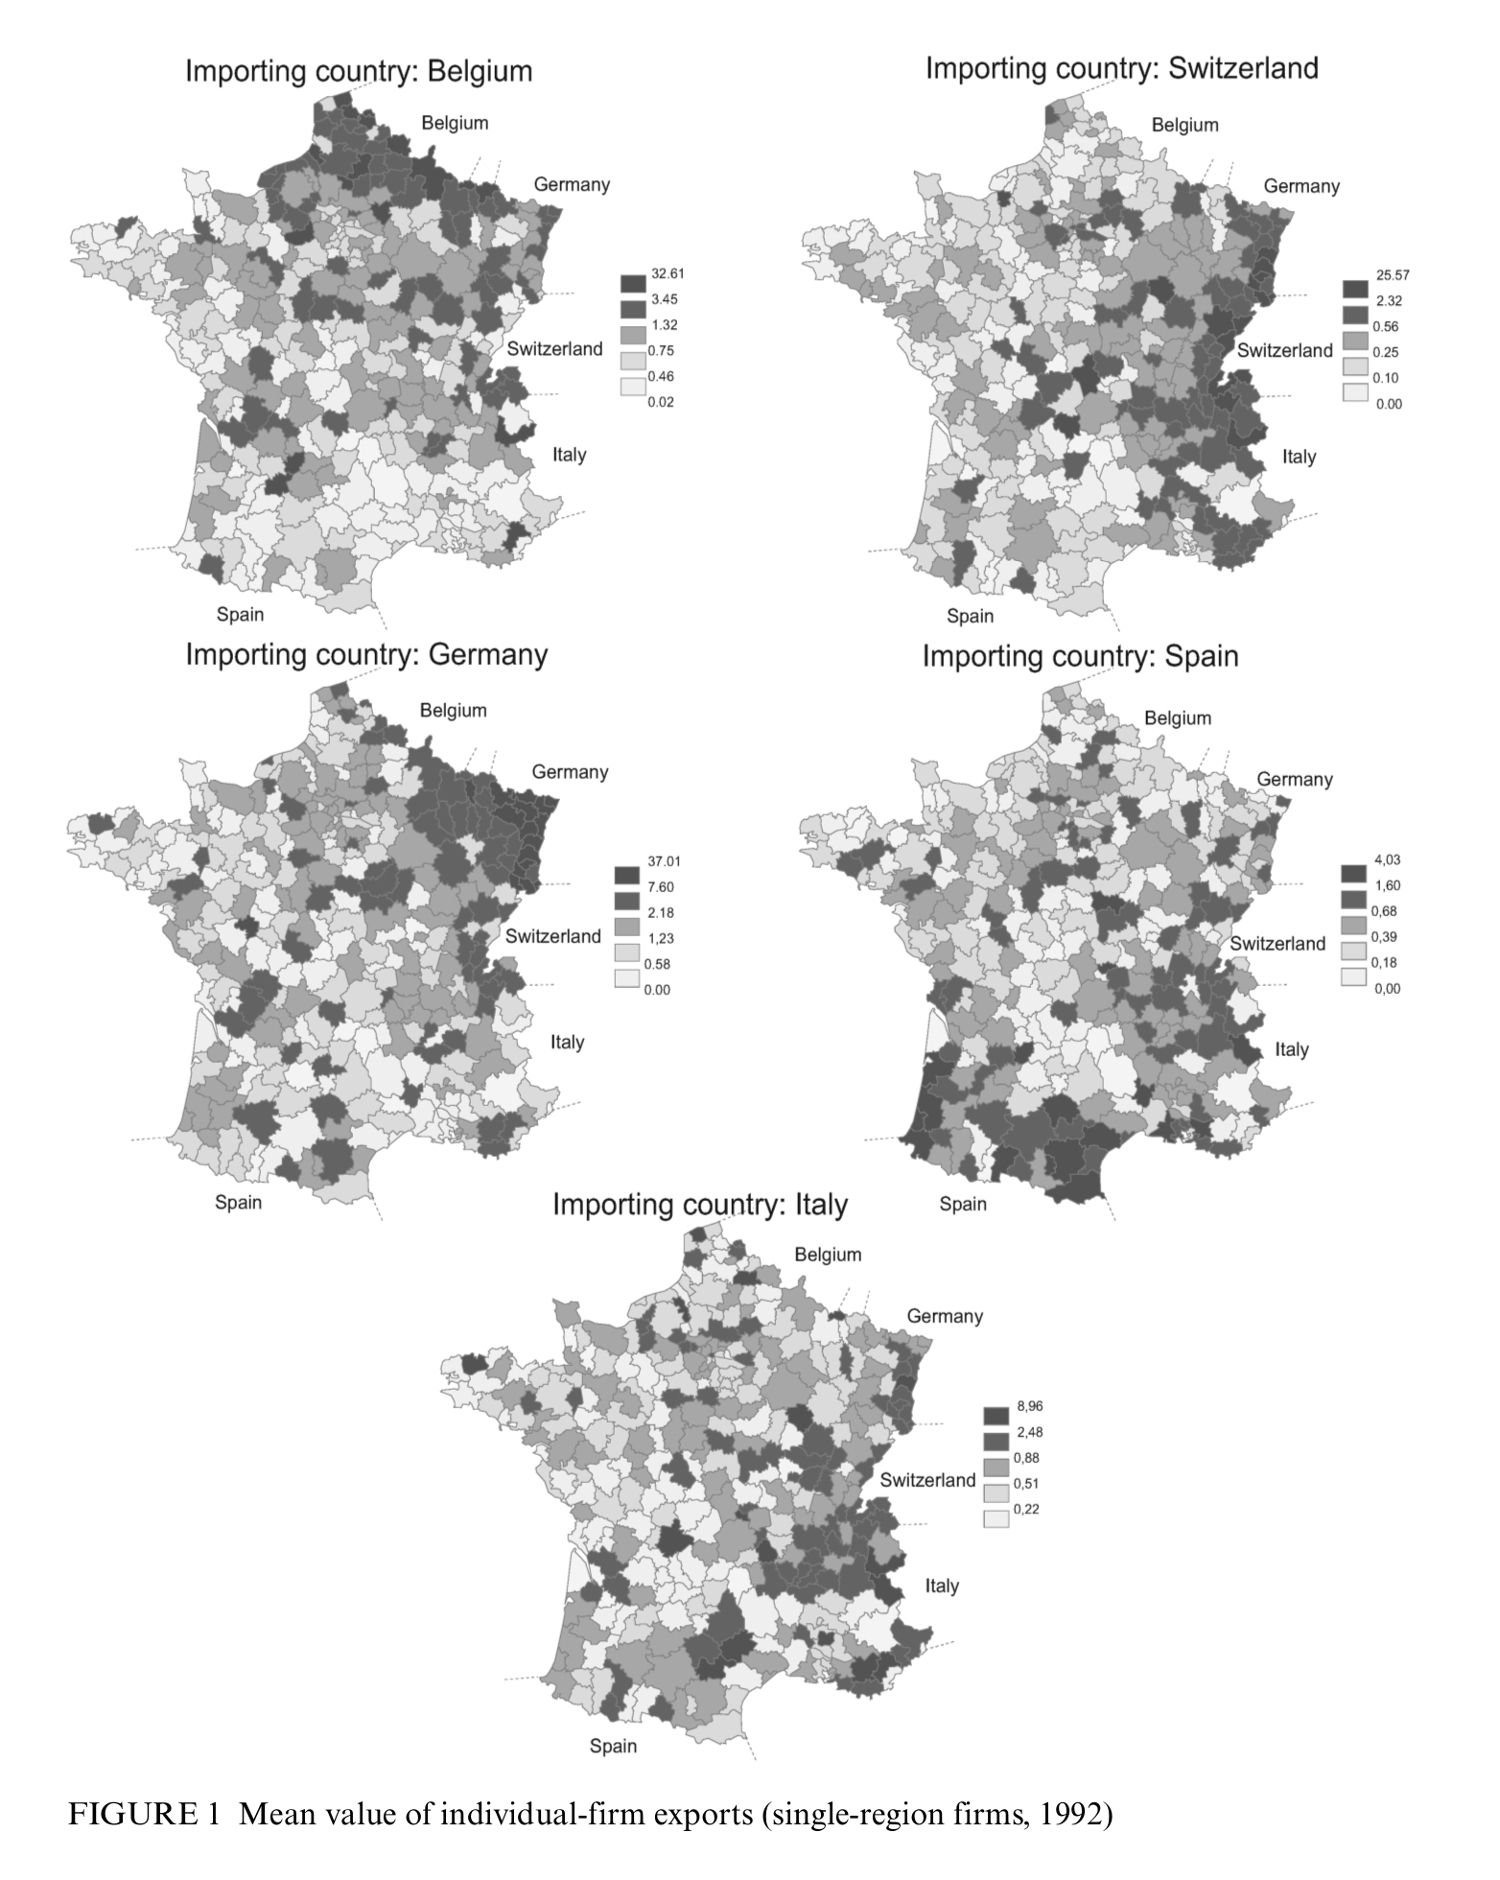
\includegraphics[scale=.1]{croezet_koenig1}
  \end{figure}  
\end{frame}
%--------------------------------------
%--------------------------------------
\begin{frame}{Mean value of individual firm exports}
\framesubtitle{Croezet and Koenig, 2010}
  \begin{figure}\centering
    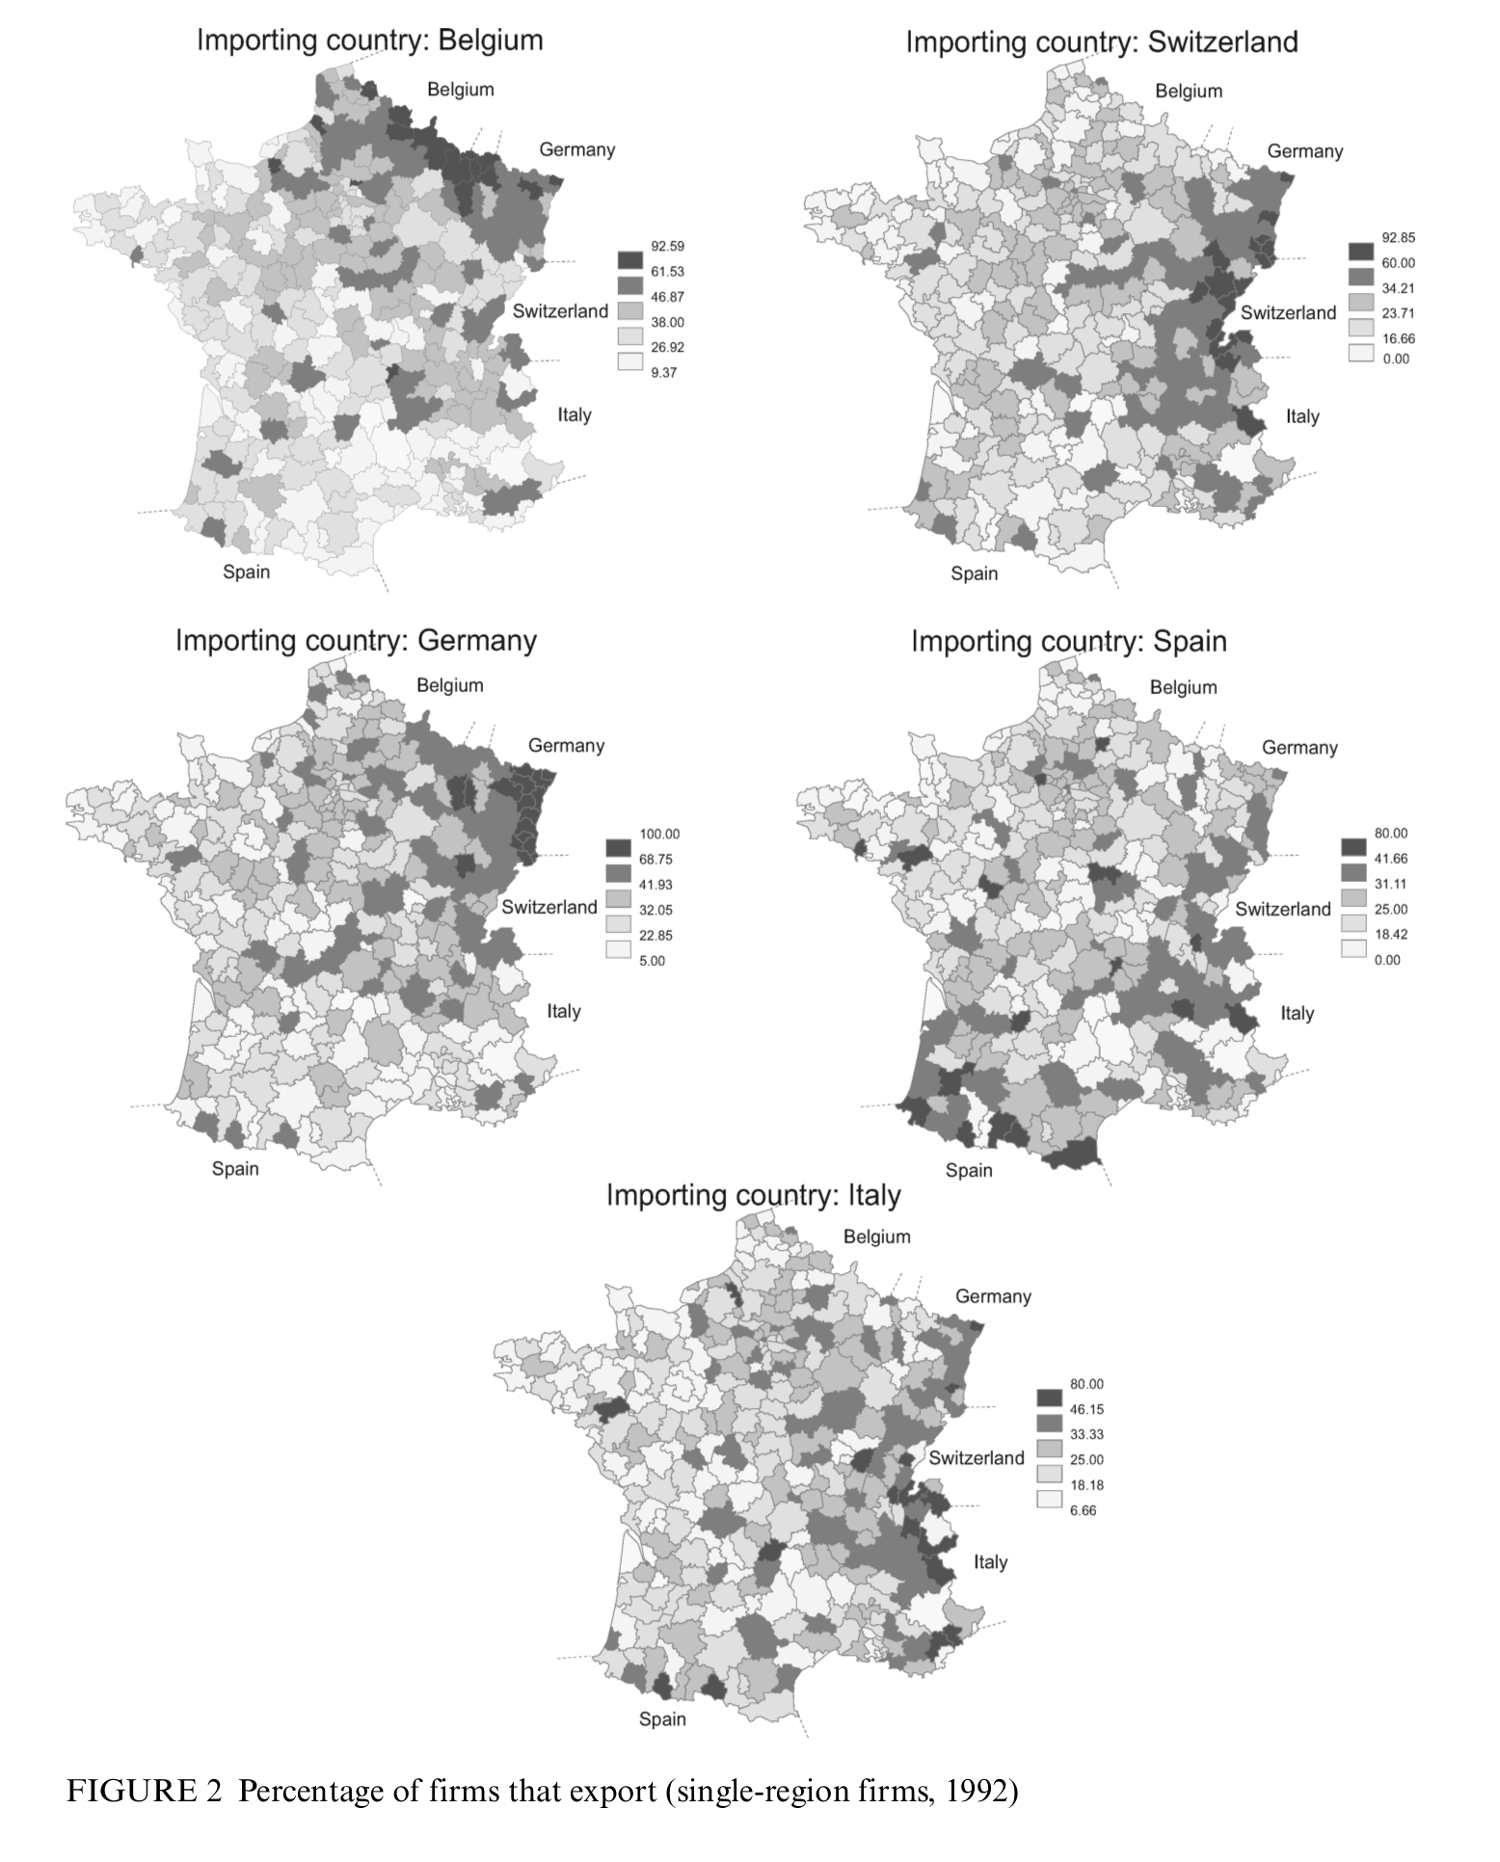
\includegraphics[scale=.1]{croezet_koenig2}
  \end{figure}  
\end{frame}
%--------------------------------------

%--------------------------------------
\begin{frame}{World trade relative to GDP over time}
\framesubtitle{source: World Bank Development Indicators}
  \begin{figure}
    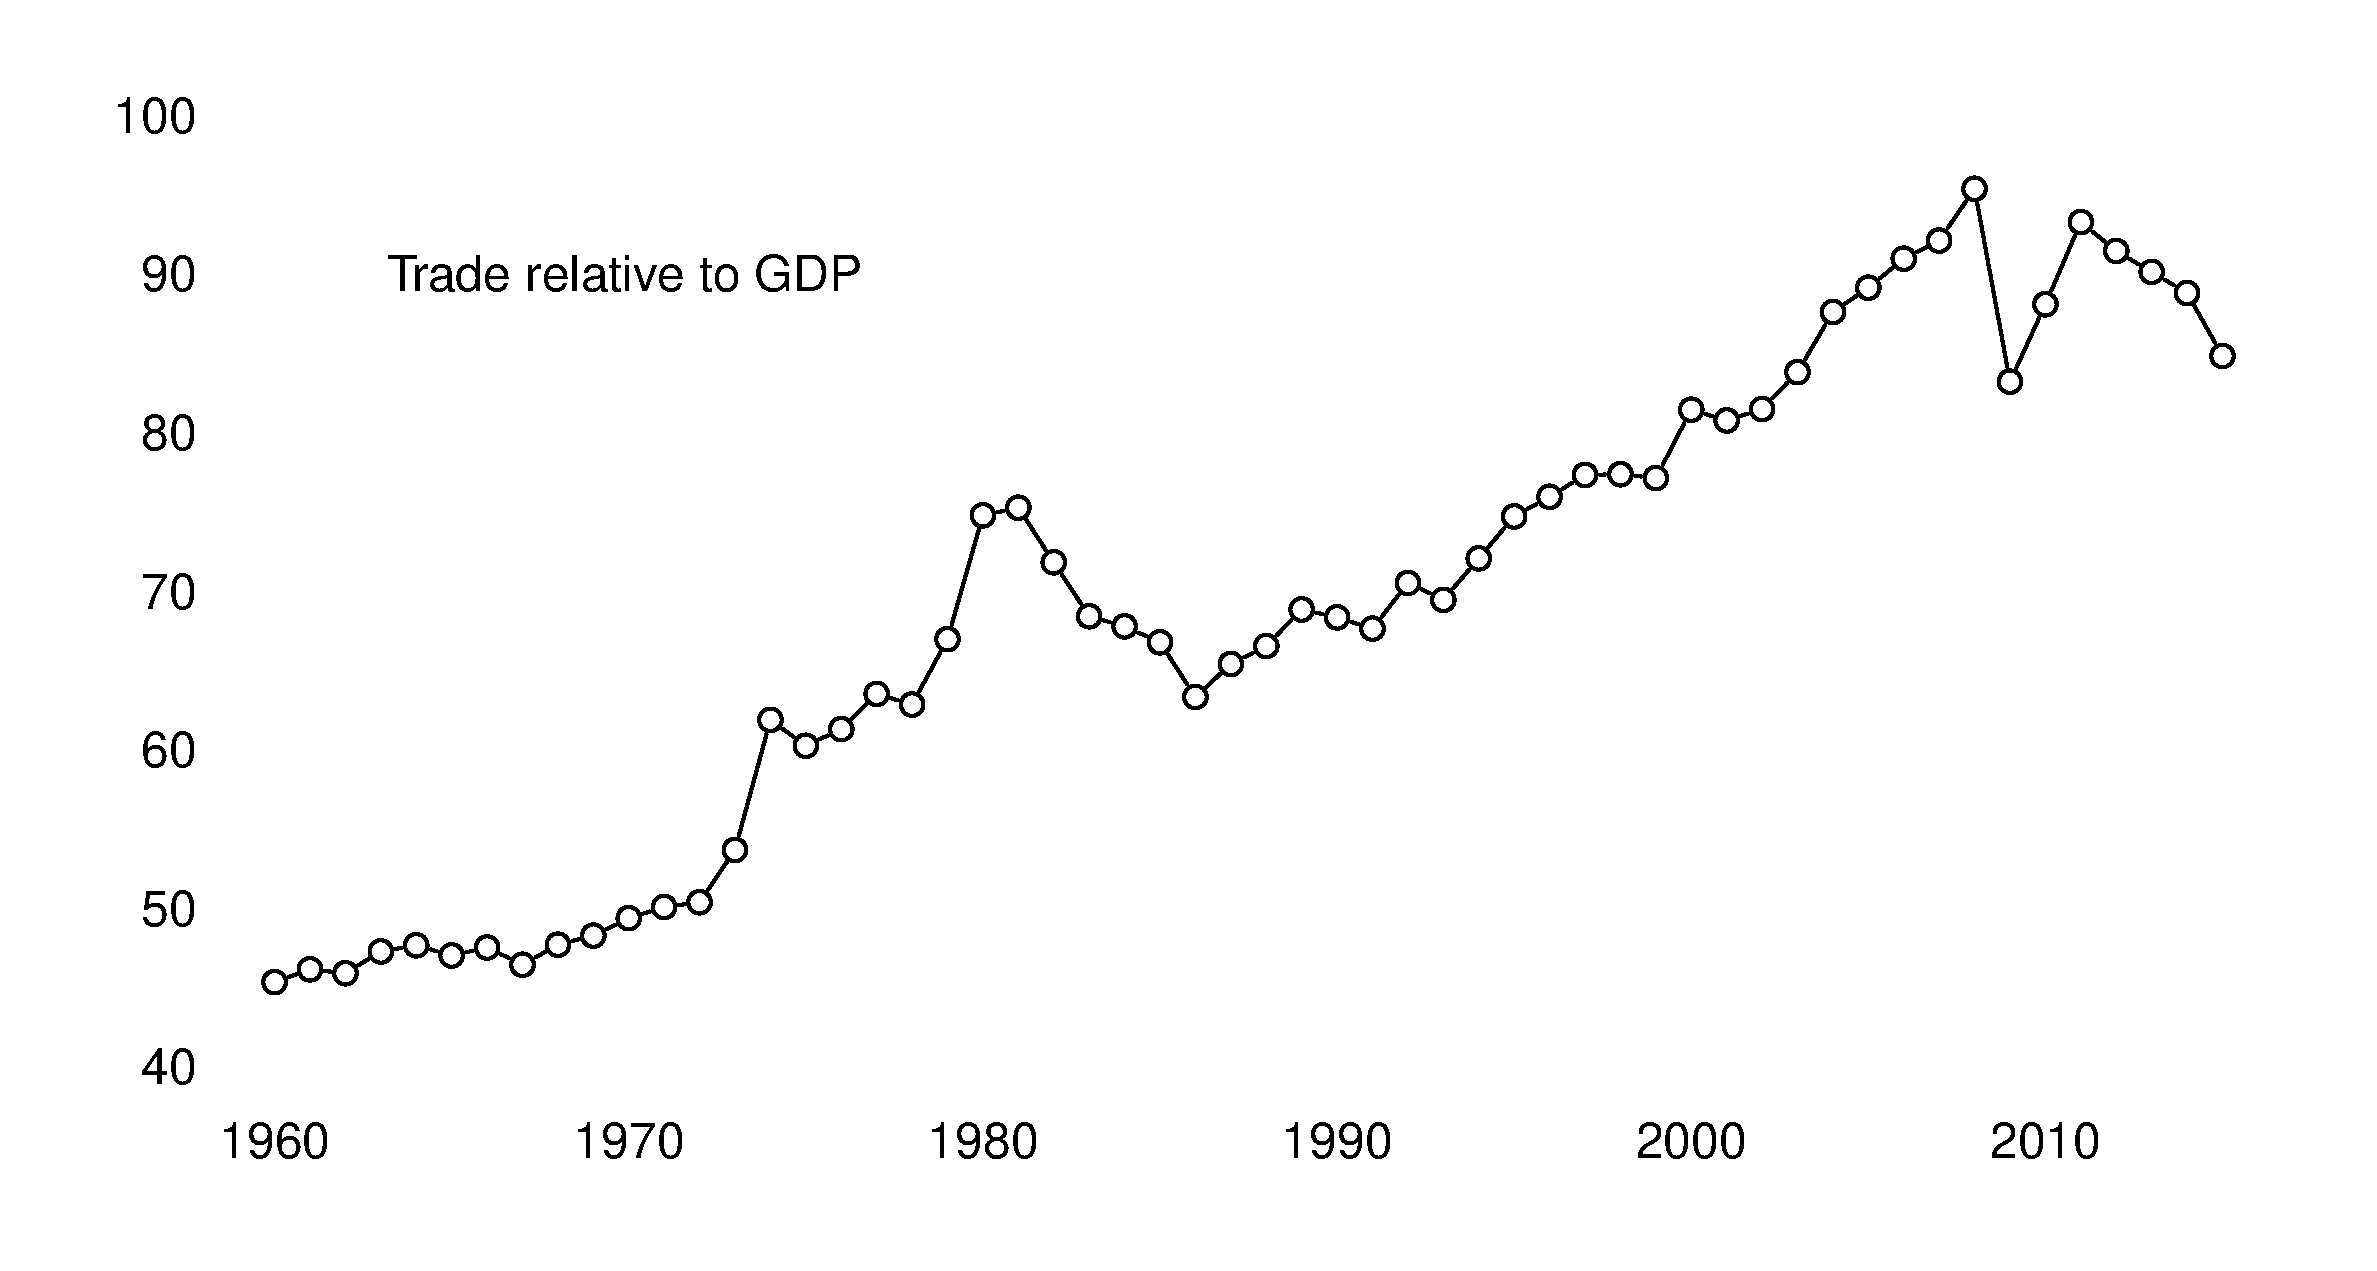
\includegraphics[scale=.25]{world_trade2}
  \end{figure}  
\end{frame}
%--------------------------------------


%--------------------------------------
\begin{frame}
  A number of technological improvements have reduced the costs of trade, or relative distance, in the past half-century
  \begin{itemize}
    \item Containerisation; lowered costs and shipping time of manufactured goods
    \item Commercial jet air transport costs fell by 90\% between 1955-2004
    \medskip
    \item International telephone costs per minute fell by 95\% between 1980-2010
    \item Internet-based communication increases bandwith of long-distance information flows    
  \end{itemize}
\end{frame}
%--------------------------------------

%--------------------------------------
\begin{frame}
  Other factors influencing trade volumes include
  \begin{itemize}
    \item Geography
    \begin{itemize}
      \item Port availability and lack of mountain barriers facilitate transport
    \end{itemize}
    \medskip
    \item Cultural distance
    \begin{itemize}
      \item Cultural ties often correlated with economic ties
      \item Different cultures could inhibit communication, generate misunderstandings, clashes in negotiation style etc.
    \end{itemize}
    \medskip
    \item Multinationals
    \begin{itemize}
      \item Imports/exports between company's divisions
      \item Synchronisation costs
    \end{itemize}
    \medskip
    \item Borders
    \begin{itemize}
      \item Crossing borders involves bureaucracy and possibly tariffs
    \end{itemize}    
  \end{itemize}  
\end{frame}
%--------------------------------------

%--------------------------------------
\begin{frame}
  \begin{figure}\centering
    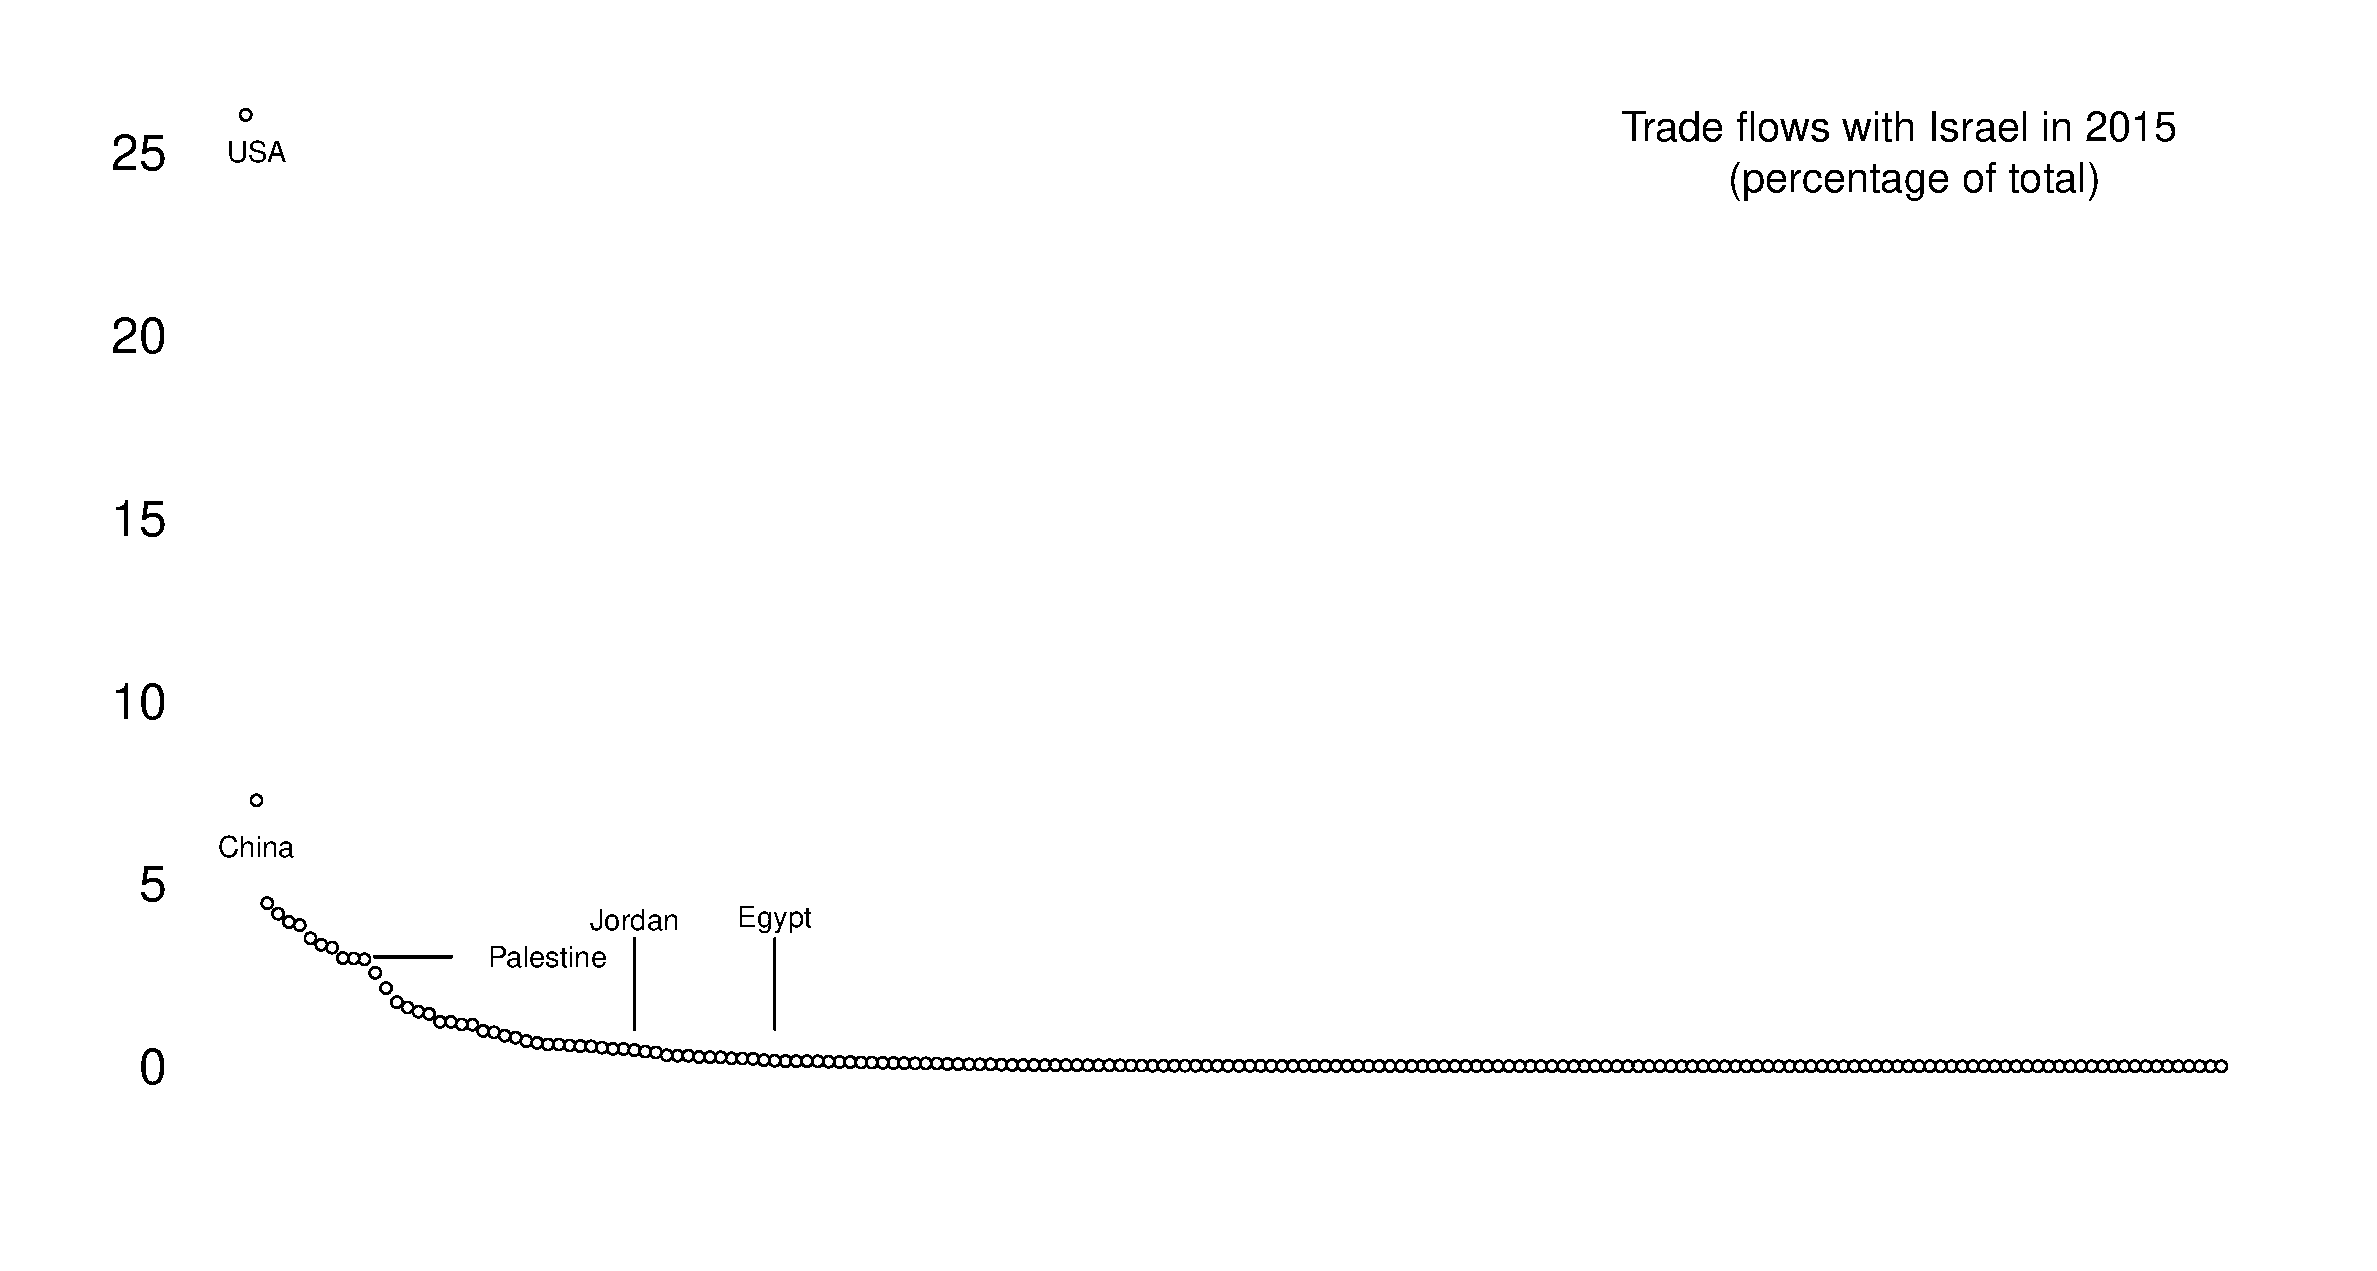
\includegraphics[scale=.3]{israel}
  \end{figure}
\end{frame}
%--------------------------------------

%--------------------------------------
\begin{frame}
  Although distance is accounted for using a simple geographic measure it can proxy for factors such as
  \begin{enumerate}
    \item Similar language
    \item Cultural affinity
    \item Contiguity
  \end{enumerate}
\end{frame}
%--------------------------------------

%--------------------------------------
\begin{frame}
  The original formulation of the gravity model simply describes an empirical relationship. 
  Of course economists could not resist to derive the equation formally.
  Let's assume that $s_{ij}$ is the share of $M_j$ that is spent on goods from country $i$, we get
  \begin{align*}
    T_{ij} = s_{ij}M_j
  \end{align*}
  We know about $s$ that
  \begin{itemize}
    \item $0 \geq s \leq 1 $
    \item Increase if $i$ produces wide variety of goods; large $n_i$
    \item Increase if goods from $i$ are perceived to be of high quality; large $\mu_i$
    \item Decrease due to trade barriers such as distance $D_{ij}$
  \end{itemize}
\end{frame}
%--------------------------------------

%--------------------------------------
\begin{frame}
  $s$ can be written as
  \begin{align*}
    s_{ij} = \frac{g(n_i,\mu_i,D_{ij})}{\sum_l g(n_l,\mu_l,D_{lj})}
  \end{align*}
  \medskip
  A specific $g()$ is required and here we will use one that let's both $n$ and $\mu$ vary across countries
  \begin{itemize}
    \item Also assume that different goods are of the same average quality and subject to same transport costs
  \end{itemize}
  \begin{align*}
    g() = n_i (p_{ij}/\mu_{ij})^{1-\sigma}
  \end{align*}
  $\sigma$ is elasticity of substitution  
\end{frame}
%--------------------------------------

%--------------------------------------
\begin{frame}
  Next step is to link the delivery price to the price in the country of origin and the transportation costs. 
  The following relationship is assumed\footnote{Note that the delivery price is quality-adjusted.}
  \begin{align*}
    \frac{p_{ij}}{\mu_{ij}} = \left(\frac{p_i}{\mu_i}\right)D_{ij}^\delta
  \end{align*}
  The origin price $p_i$ is also know as the free-on-board price and in this model it varies according to the quality of the export country's products: $\frac{p_{i}}{\mu_{i}} \approx k$\\  
  Since we can't observe $n_i$ we assume that all firms are the same size $q$
  \begin{align*}
    n_i=M_i/q
  \end{align*}  
\end{frame}
%--------------------------------------

%--------------------------------------
\begin{frame}
  Finally, defining $\theta \equiv \delta (\sigma-1) \geq 0$ we get
  \begin{align*}
    g()= \frac{M_iD^{-\theta}}{qk^{\sigma-1}}
  \end{align*}
  \medskip
  Which implies that the market share for exporter $i$ in country $j$ is given by
  \begin{align*}
    s_{ij} = M_iD_{ij}^{-\theta}R_j
  \end{align*}
  \medskip 
  Where $R_j = \frac{1}{\sum_l M_l D_{lj}^\theta}$ and captures remoteness.\\ 
  We can rewrite this into
  \begin{align*}
    T_{ij} = R_j \frac{M_i M_j}{D_{ij}^\theta}
  \end{align*}
  Note that $R_j$ replaces the gravitational constant $\alpha$
\end{frame}
%--------------------------------------

%--------------------------------------
\begin{frame}
  Concerning remoteness let's consider two dyads
  \medskip
  \begin{enumerate}
    \item Australia - New Zealand
    \begin{itemize}
      \item Distance between Sydney - Auckland: 2160 Km
      \item Combined GDP: 1.4T USD
    \end{itemize}
    \medskip
    \item Spain - Hungary
    \begin{itemize}
      \item Distance between Madrid - Budapest: 1982 Km
      \item Combined GDP: 1.3T USD
    \end{itemize}
  \end{enumerate}
  \medskip  
  What would we expect in terms of trade flow for each dyad?
\end{frame}
%--------------------------------------

%--------------------------------------
\begin{frame}
  Trade flows per dyad in 2015
  \begin{enumerate}
    \item Australia - New Zealand: 10.9B USD
    \item Spain - Hungary: 4.2B USD
  \end{enumerate}  
\end{frame}
%--------------------------------------

%--------------------------------------
\begin{frame}
  The US economy
  \begin{itemize}
    \item Exports about 2.1T USD per year, accounting for 13.8\% of GDP
    \item Exports support about 6.8 million jobs
  \end{itemize}
  \medskip
  What percentage of US firms exports?
\end{frame}
%--------------------------------------


%--------------------------------------
\begin{frame}
  Of 30 million US companies, less than 1 \% exports, according to US sources
  \begin{itemize}
    \item Of these companies, 58\% exports to only one country
  \end{itemize}
  \medskip
  OECD figures show that about 4.5\% of US firms export, in the EU the average is 6\%.
\end{frame}
%--------------------------------------

%--------------------------------------
\begin{frame}{}
\framesubtitle{}
  \begin{figure}
    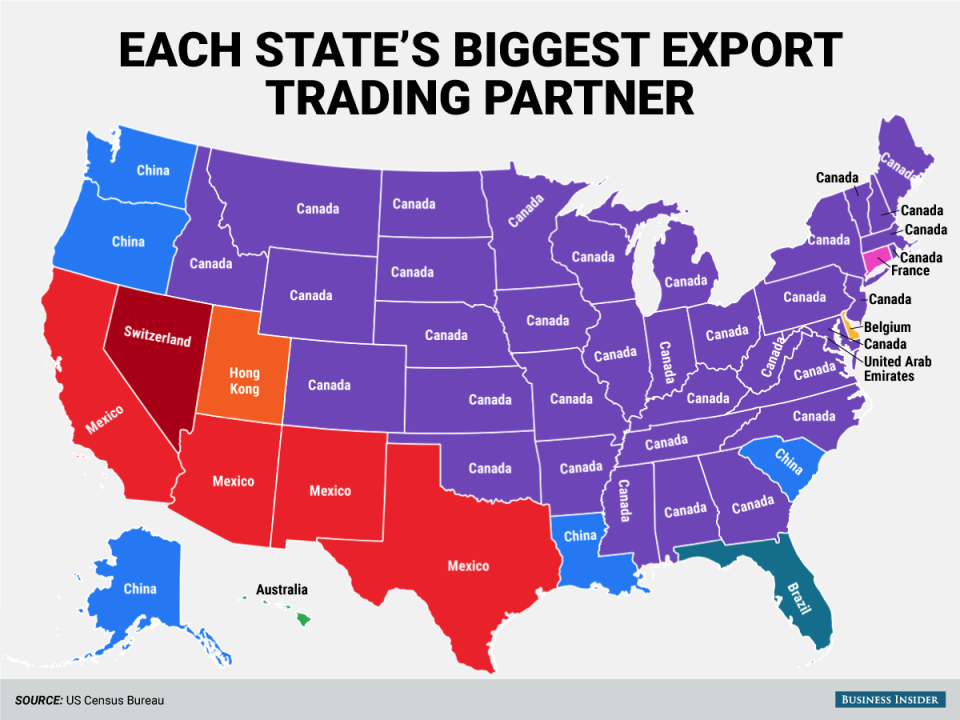
\includegraphics[scale=.3]{state_exports}
  \end{figure}  
\end{frame}
%--------------------------------------

%--------------------------------------
\begin{frame}{}
\framesubtitle{}
  \begin{figure}
    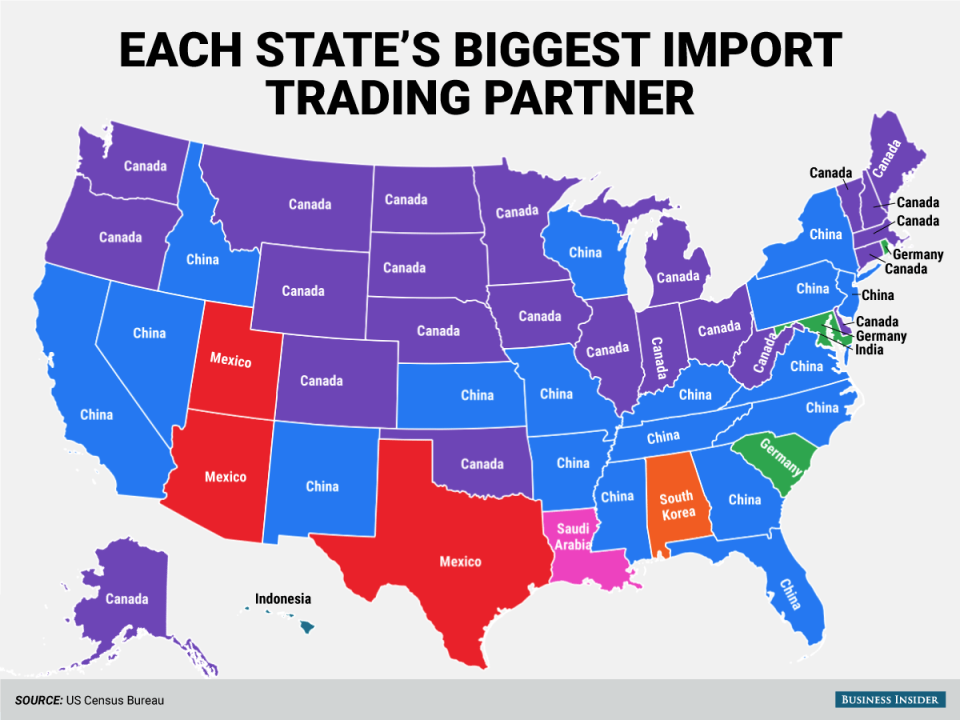
\includegraphics[scale=.3]{state_imports}
  \end{figure}  
\end{frame}
%--------------------------------------

%--------------------------------------
\begin{frame}
  USA is Canada's main trade partner: 67.7\% of total trade in 2015.
  This is probably due to 
  \begin{itemize}
    \item Similarities in terms of language, culture, history
    \item As well as small distance between countries
  \end{itemize}
  \medskip
  Border are associated with trade reduction as trade between countries is harder than within countries: this is called the Border Effect
  \begin{itemize}
    \item Within-country region-pairs are 10-20 times more likely to trade than identical pairs across countries
  \end{itemize}
\end{frame}
%--------------------------------------

%--------------------------------------
\begin{frame}{Canadian provinces and US states that trade with British Columbia}
\begin{figure}
  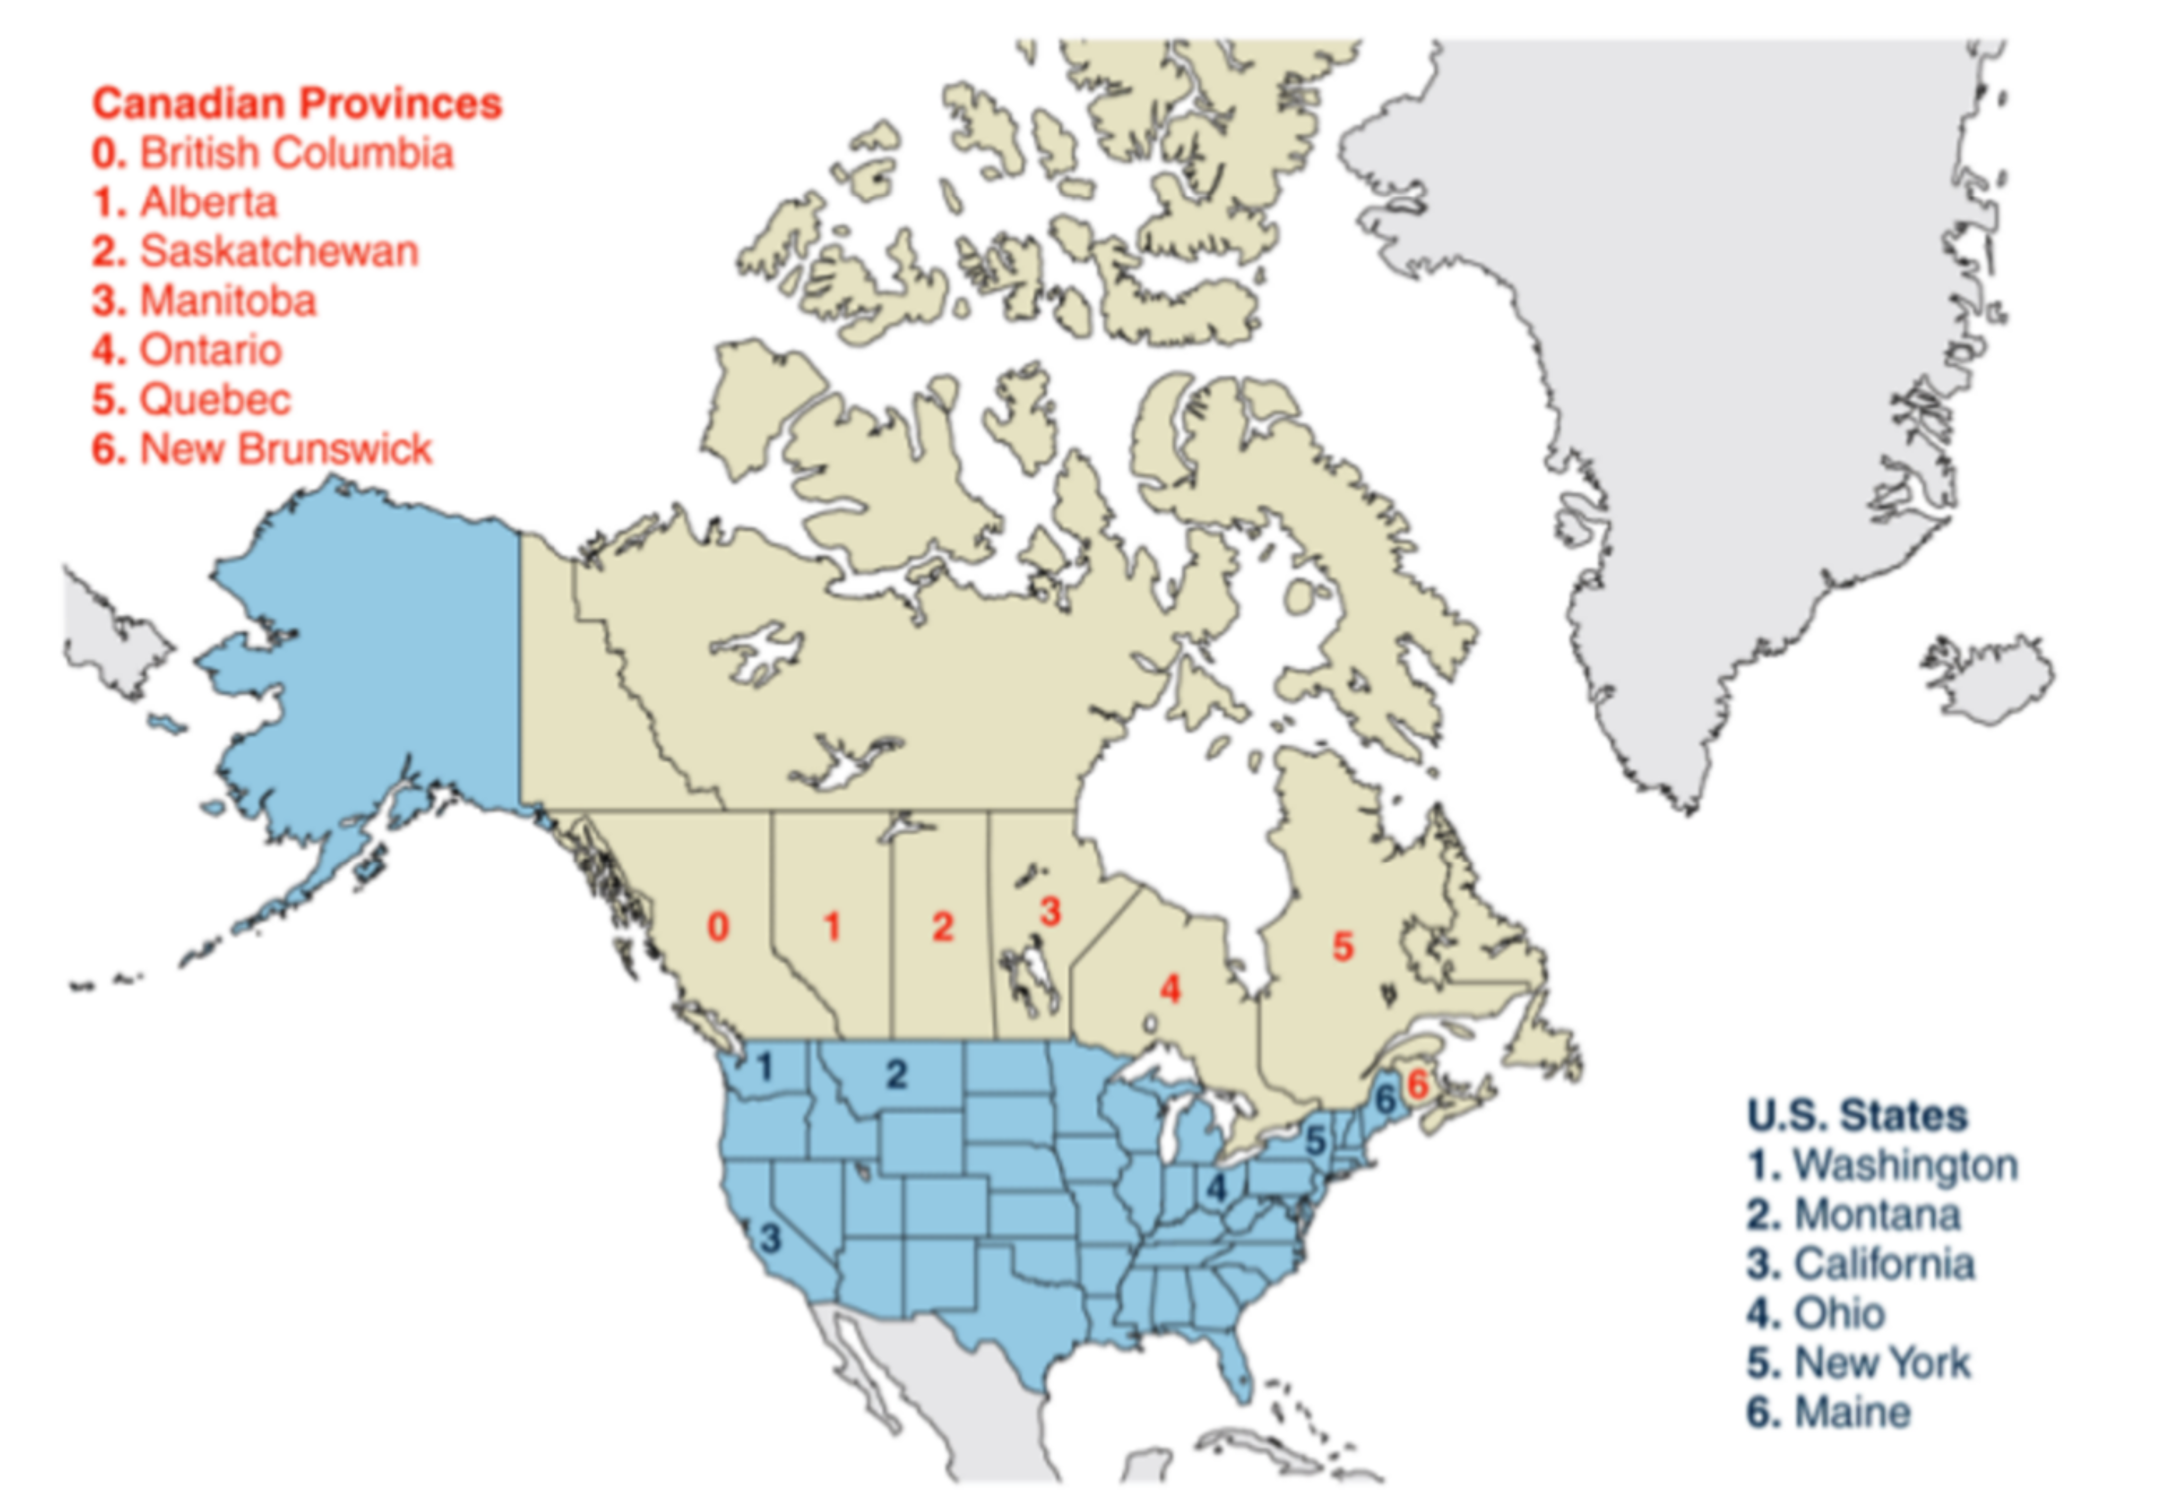
\includegraphics[scale=.5]{border_effect1}
\end{figure}  
\end{frame}
%--------------------------------------

%--------------------------------------
\begin{frame}{Canadian provinces and US states that trade with British Columbia}
\begin{figure}
  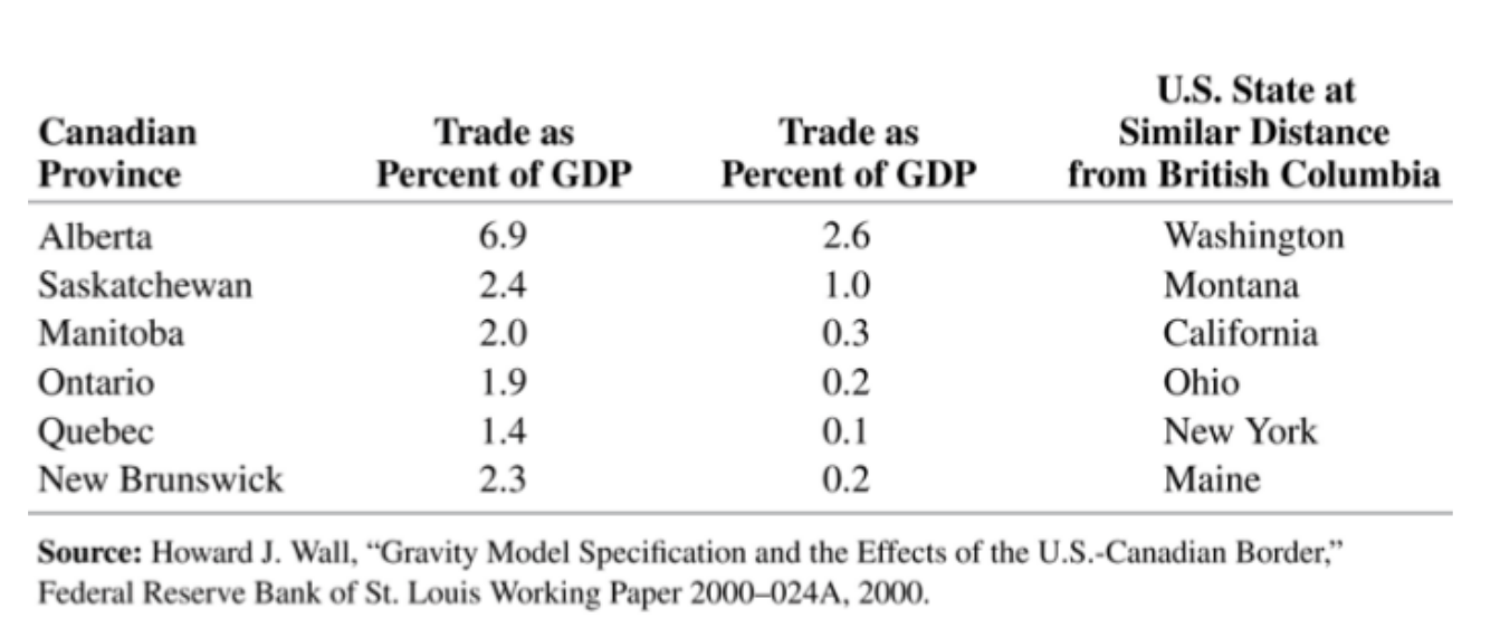
\includegraphics[scale=.7]{border_effect2}
\end{figure}  
\end{frame}
%--------------------------------------

%--------------------------------------
\begin{frame}
  A border increases both the time and costs needed to trade
  \begin{itemize}
    \item Due to bureaucracy mainly
  \end{itemize}
  \medskip
  Trade agreements can help to reduce these costs and increase trade.
  And a gravity model can help assess the effect of the trade agreement
\end{frame}
%--------------------------------------

%--------------------------------------
\begin{frame}
  North American Free Trade Agreement (NAFTA)
  \begin{itemize}
    \item Aim to eliminate barriers to trade and investments between USA, CAN, MEX
    \item Came into force in 1994    
  \end{itemize}
  \medskip
  Note: CAN economy ranks 10th in the world, MEX 15. 
\end{frame}

%--------------------------------------
\begin{frame}
  \begin{figure}\centering
    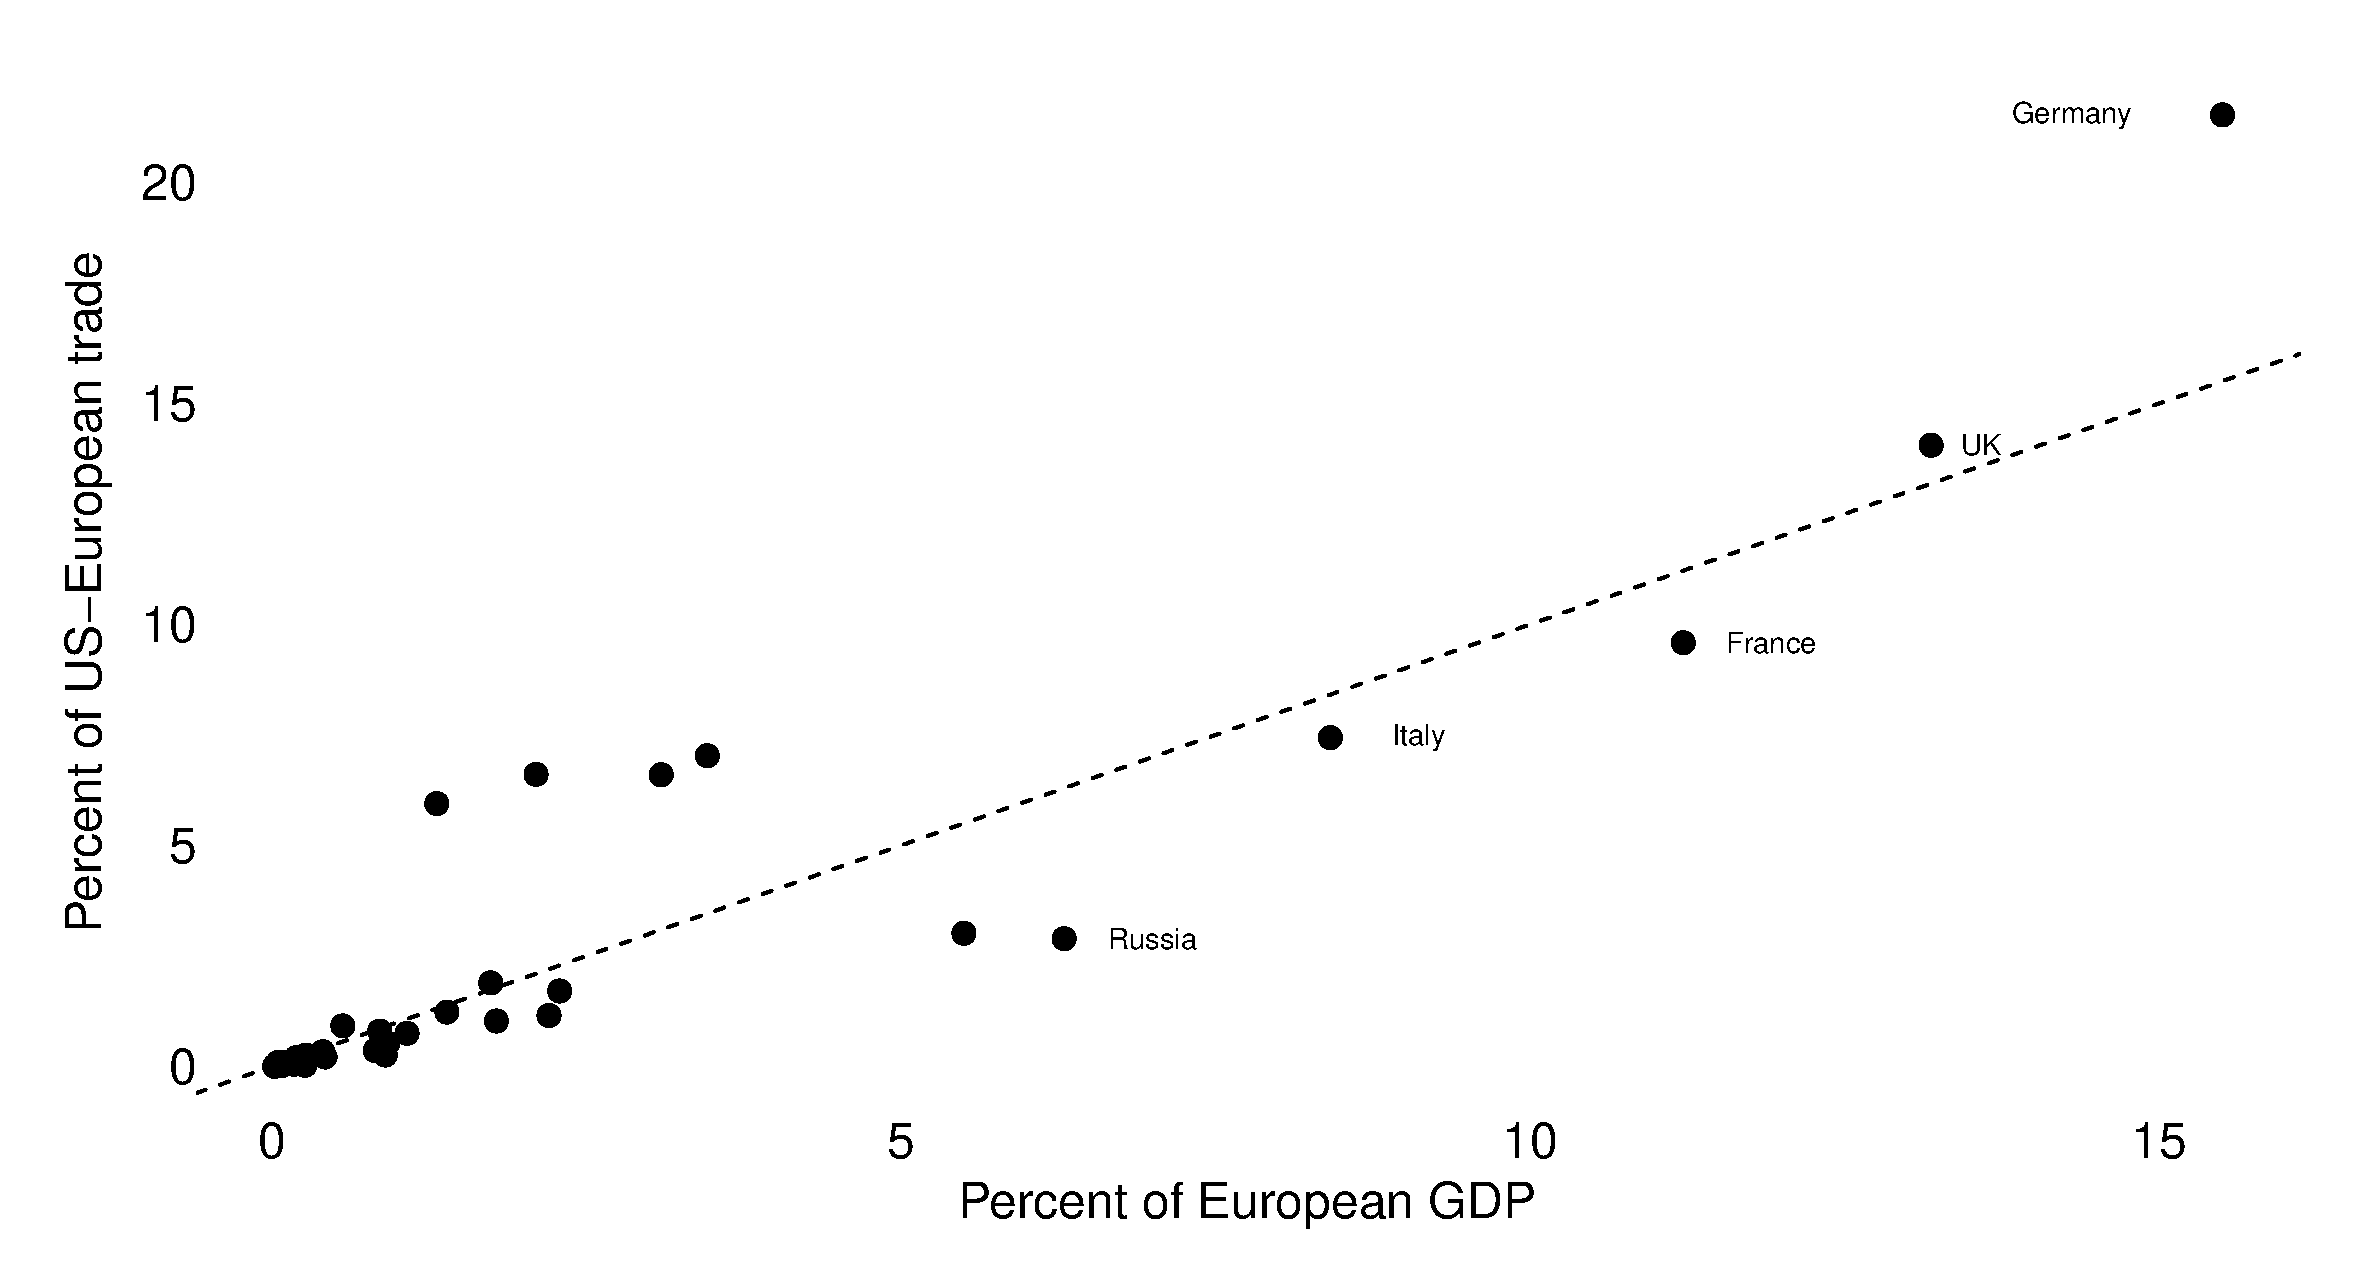
\includegraphics[scale=.25]{us_gravity}
  \end{figure}
\end{frame}
%--------------------------------------

%--------------------------------------
\begin{frame}
  \begin{figure}
    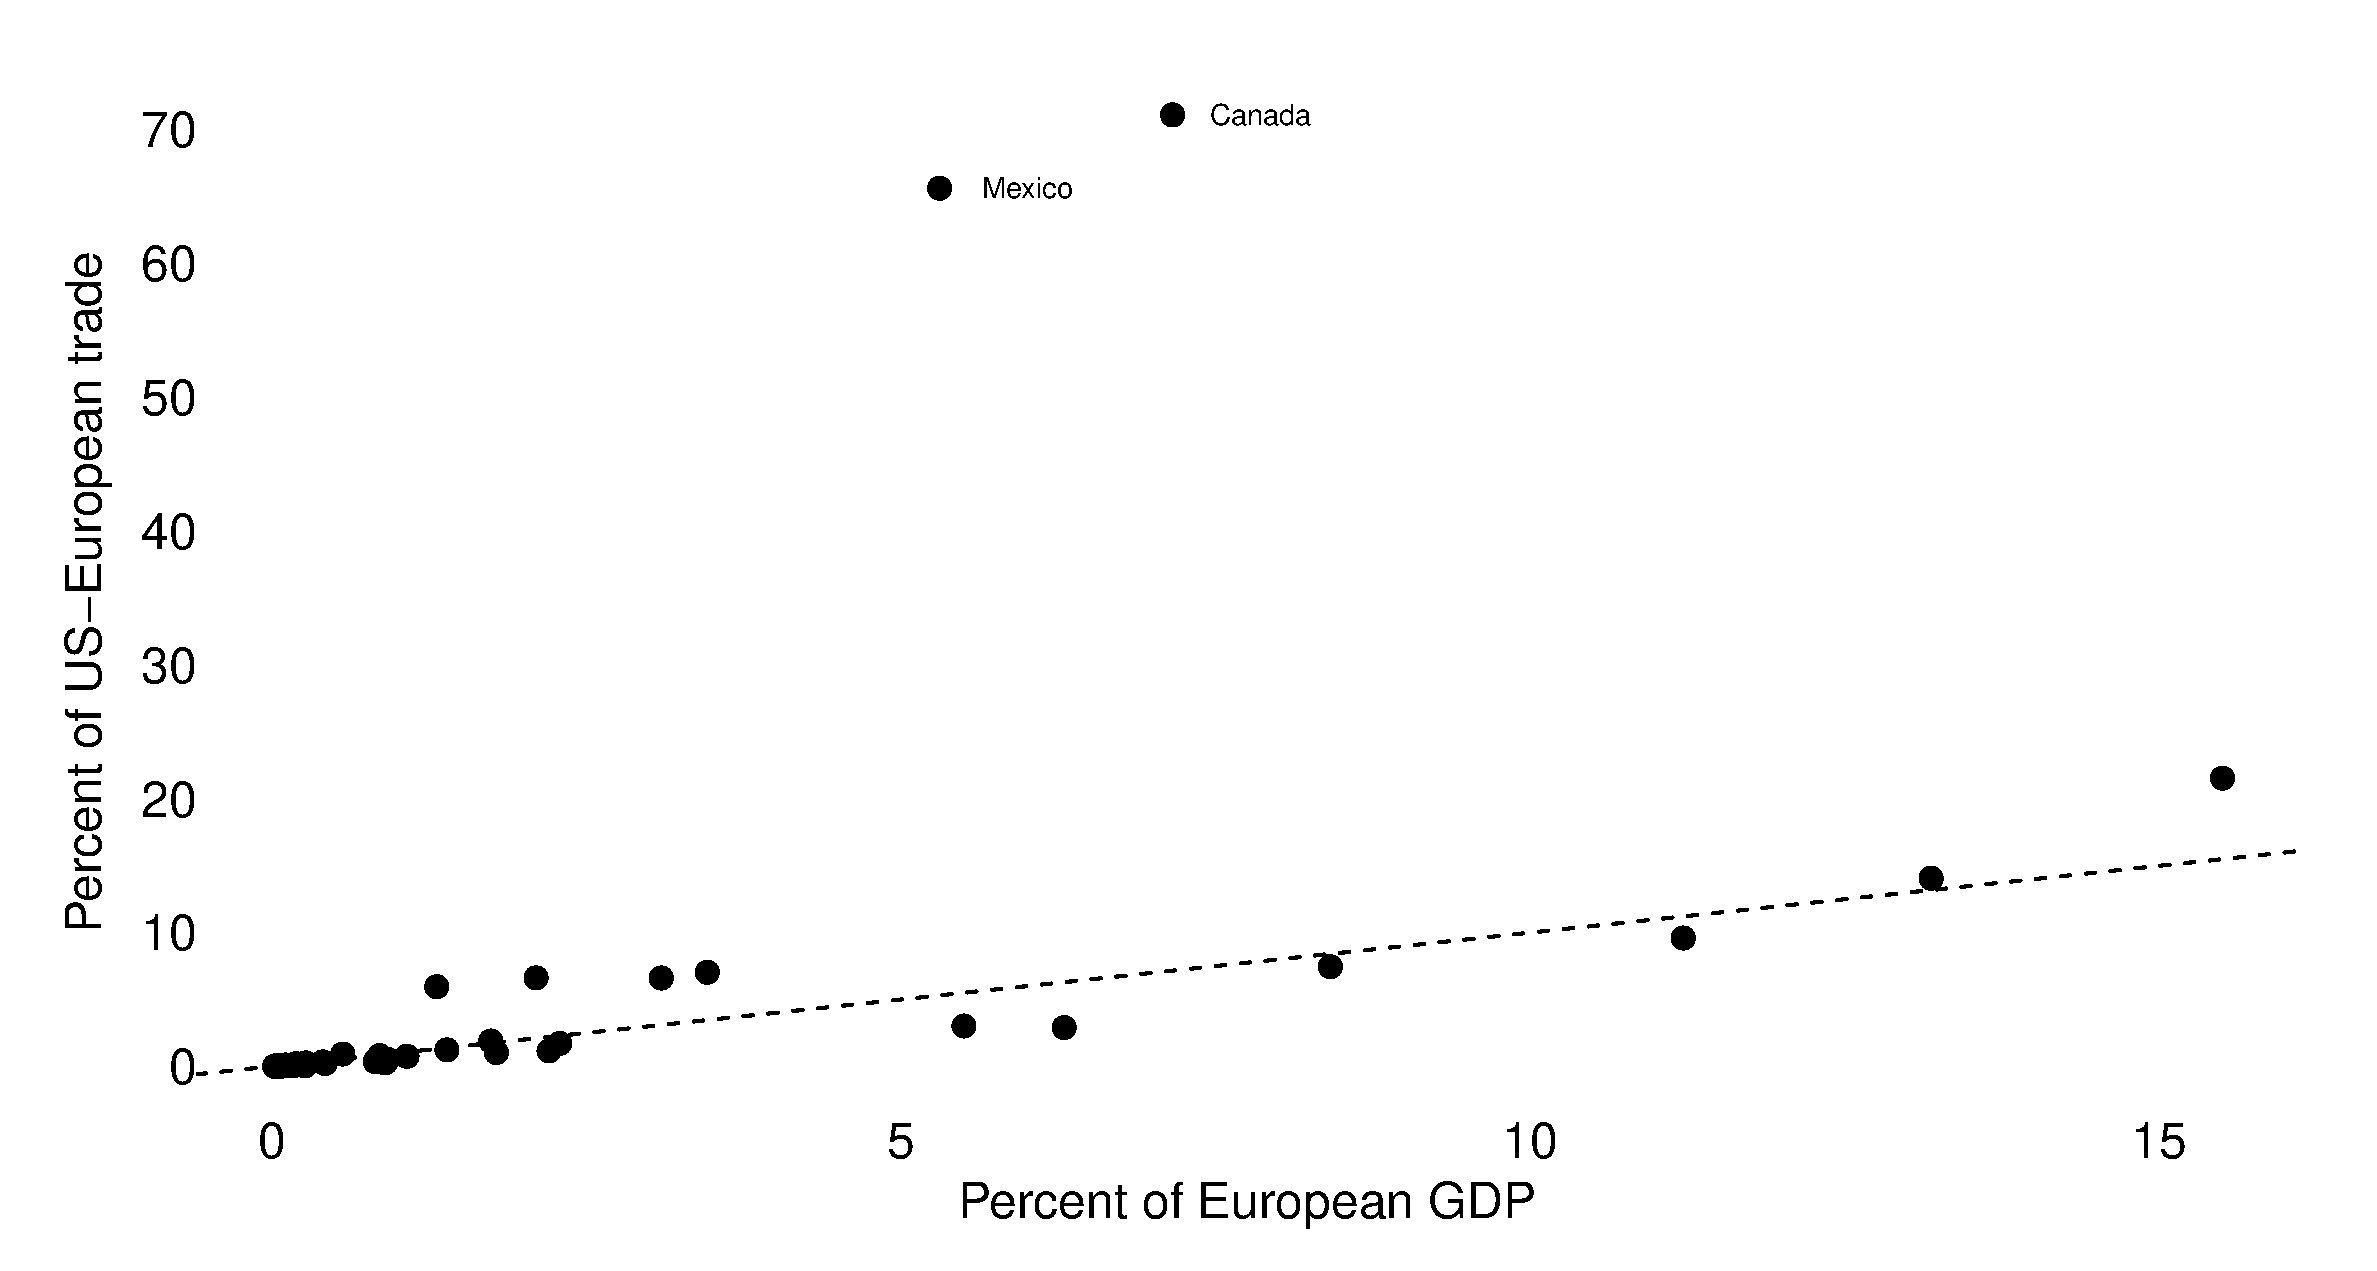
\includegraphics[scale=.3]{us_gravity2}
  \end{figure}
\end{frame}
%--------------------------------------

%--------------------------------------
\begin{frame}
  Despite technological progress in transport and communication, distance still is an important factor. 
  Not only on trade but also other flows/transactions
  \medskip
    \begin{enumerate}
      \item FDI
      \item Portfolio investment
      \item Web browsing
      \item Patent citations
    \end{enumerate}
\end{frame}
%--------------------------------------

%--------------------------------------
\begin{frame}
      Distance is a proxy for lack of information which leads to uncertainty
    \begin{itemize}
      \item Familiarity declines rapidly with distance
    \end{itemize}
    \medskip
    Additionally, distance is associated with localised tastes
    \begin{itemize}
      \item Historically determined and change slowly with experience (home bias)
    \end{itemize}
\end{frame}
%--------------------------------------

%--------------------------------------
\begin{frame}{Localised historical tastes}
\framesubtitle{source: Head and Mayer, 2013}
  \begin{figure}
    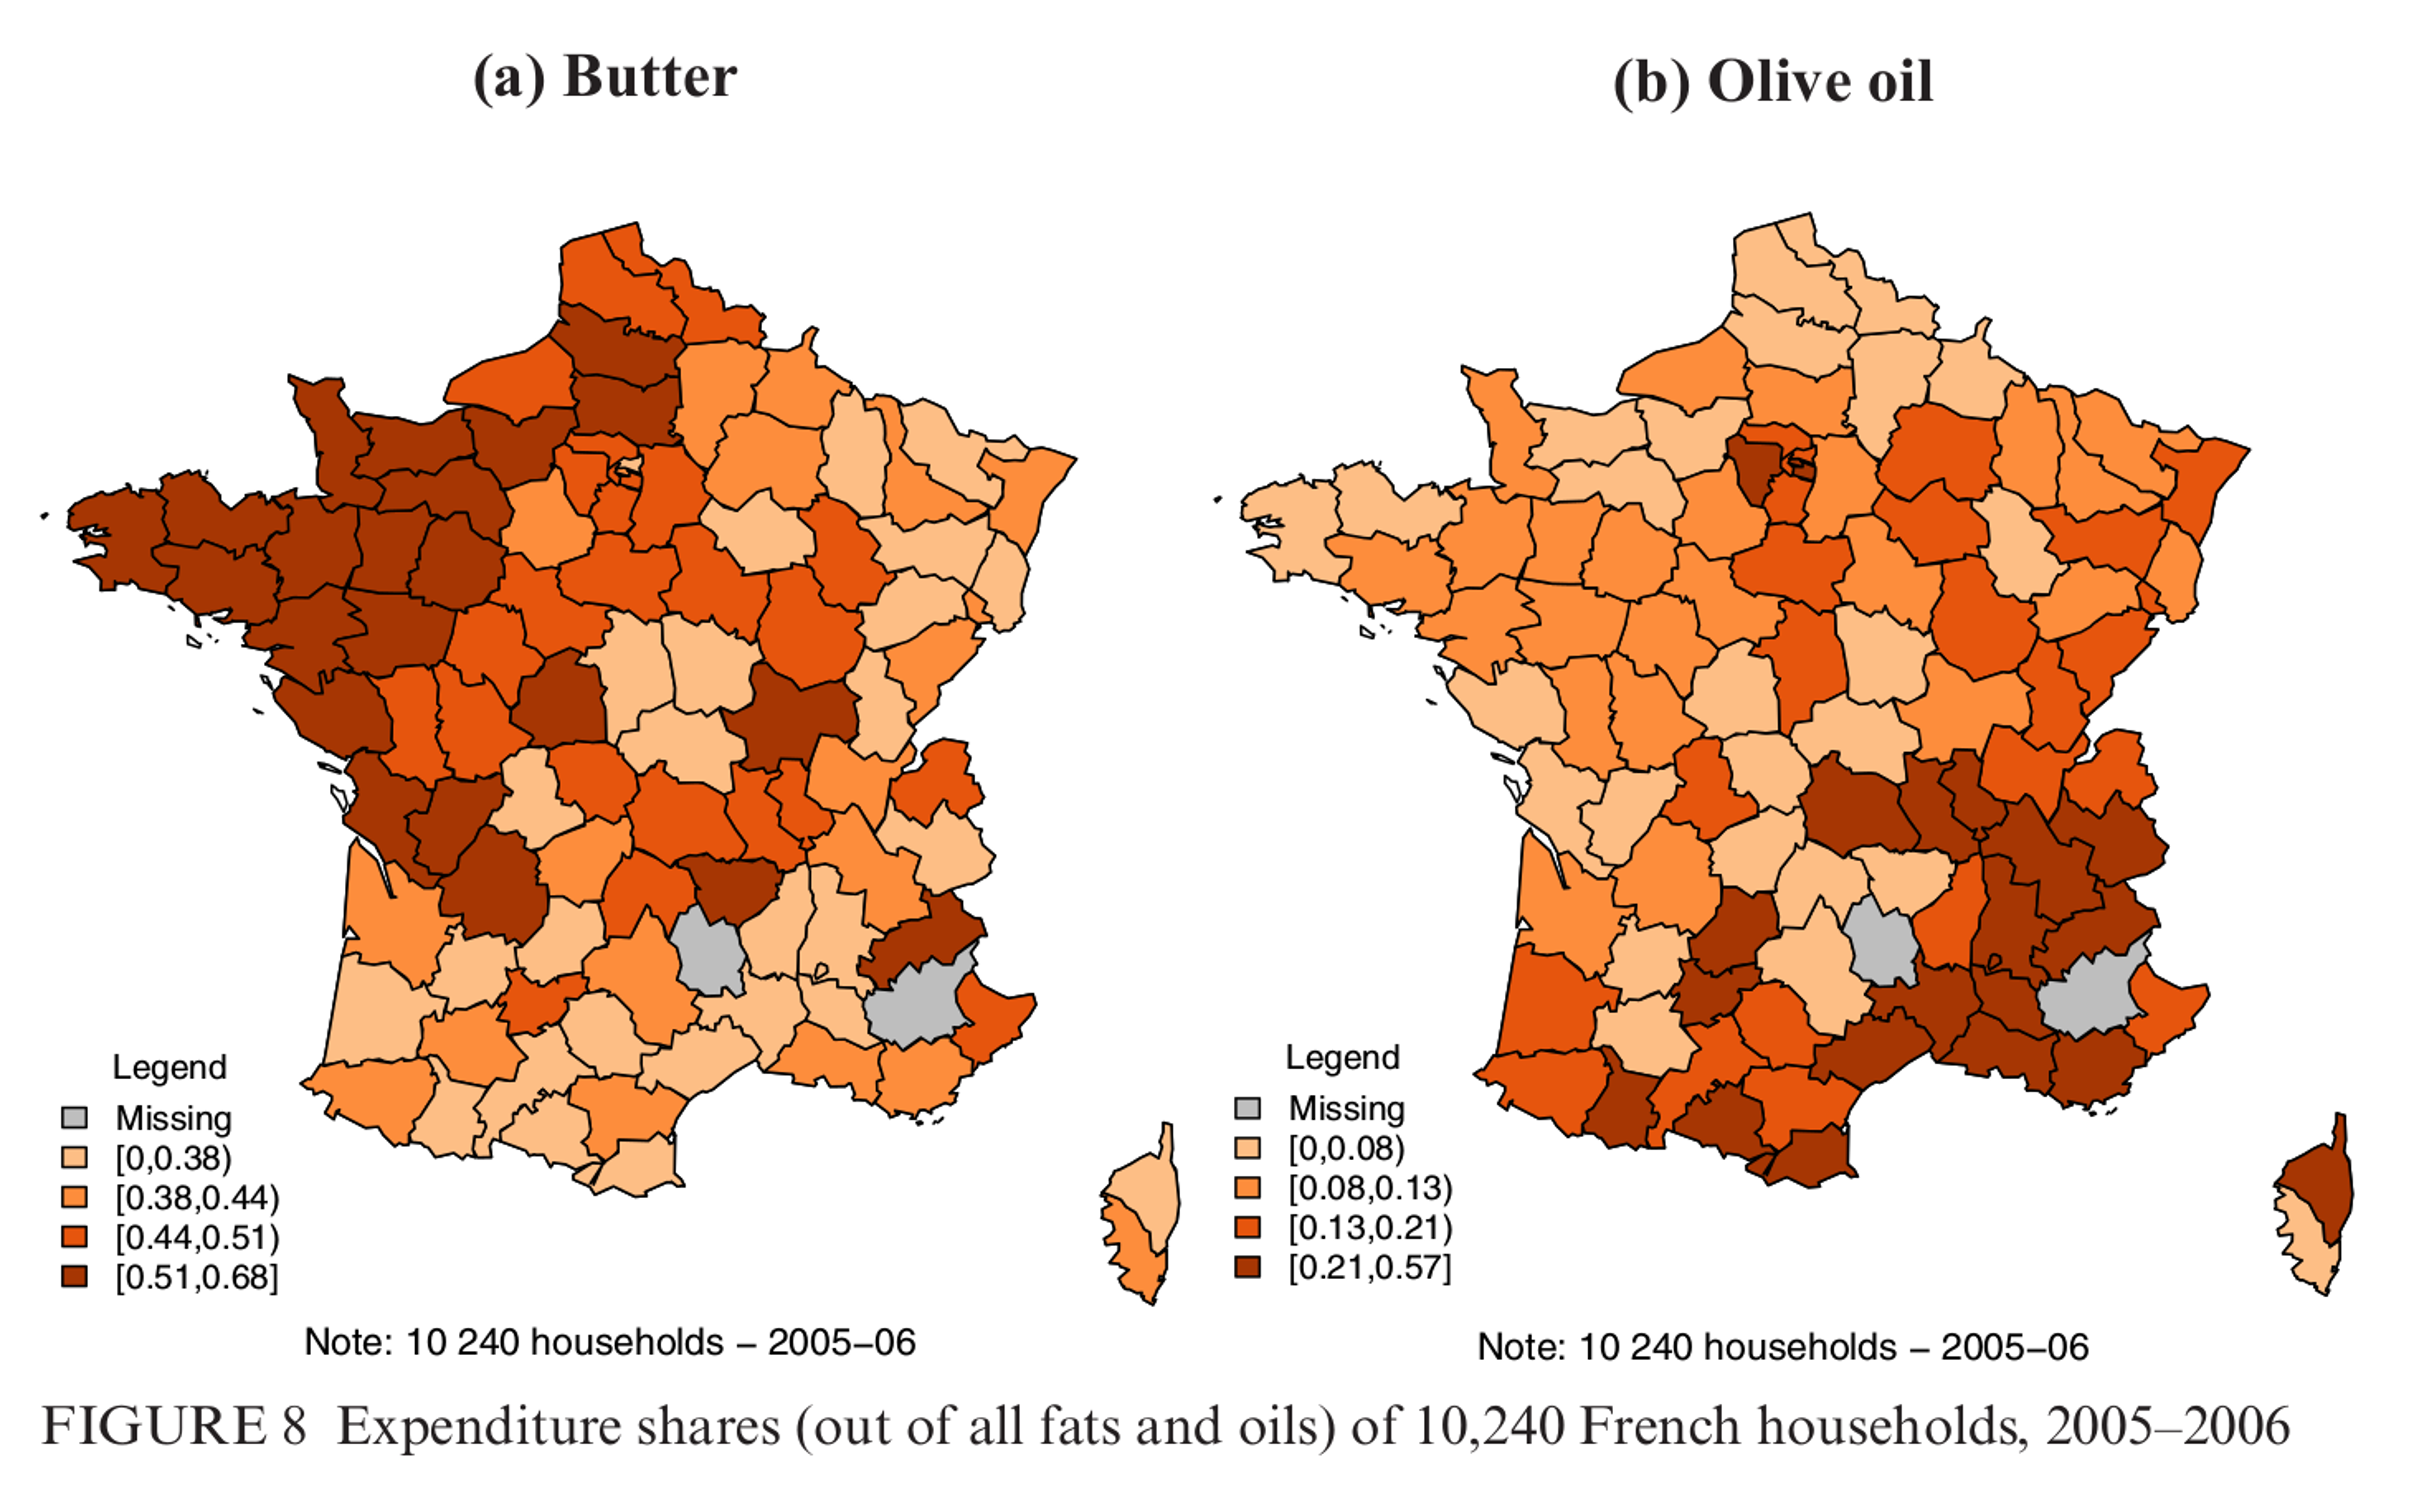
\includegraphics[scale=.5]{head_mayer2}
  \end{figure}  
\end{frame}
%--------------------------------------

%--------------------------------------
\begin{frame}
  There is some empirical evidence that suggests there are stronger trade links between metropole and former colonies
    \begin{itemize}
      \item Quebec and France, Canada and UK
    \end{itemize}
    \medskip
    Nonetheless, there is a steady decline in trade 
    \begin{itemize}
      \item between colonial power and colony
      \item between colonies of same colonial power
    \end{itemize}
\end{frame}
%--------------------------------------

%--------------------------------------
\begin{frame}{"The erosion of colonial trade linkages after independence"}
\framesubtitle{Head et al. (2010)}
  \begin{figure}\centering
    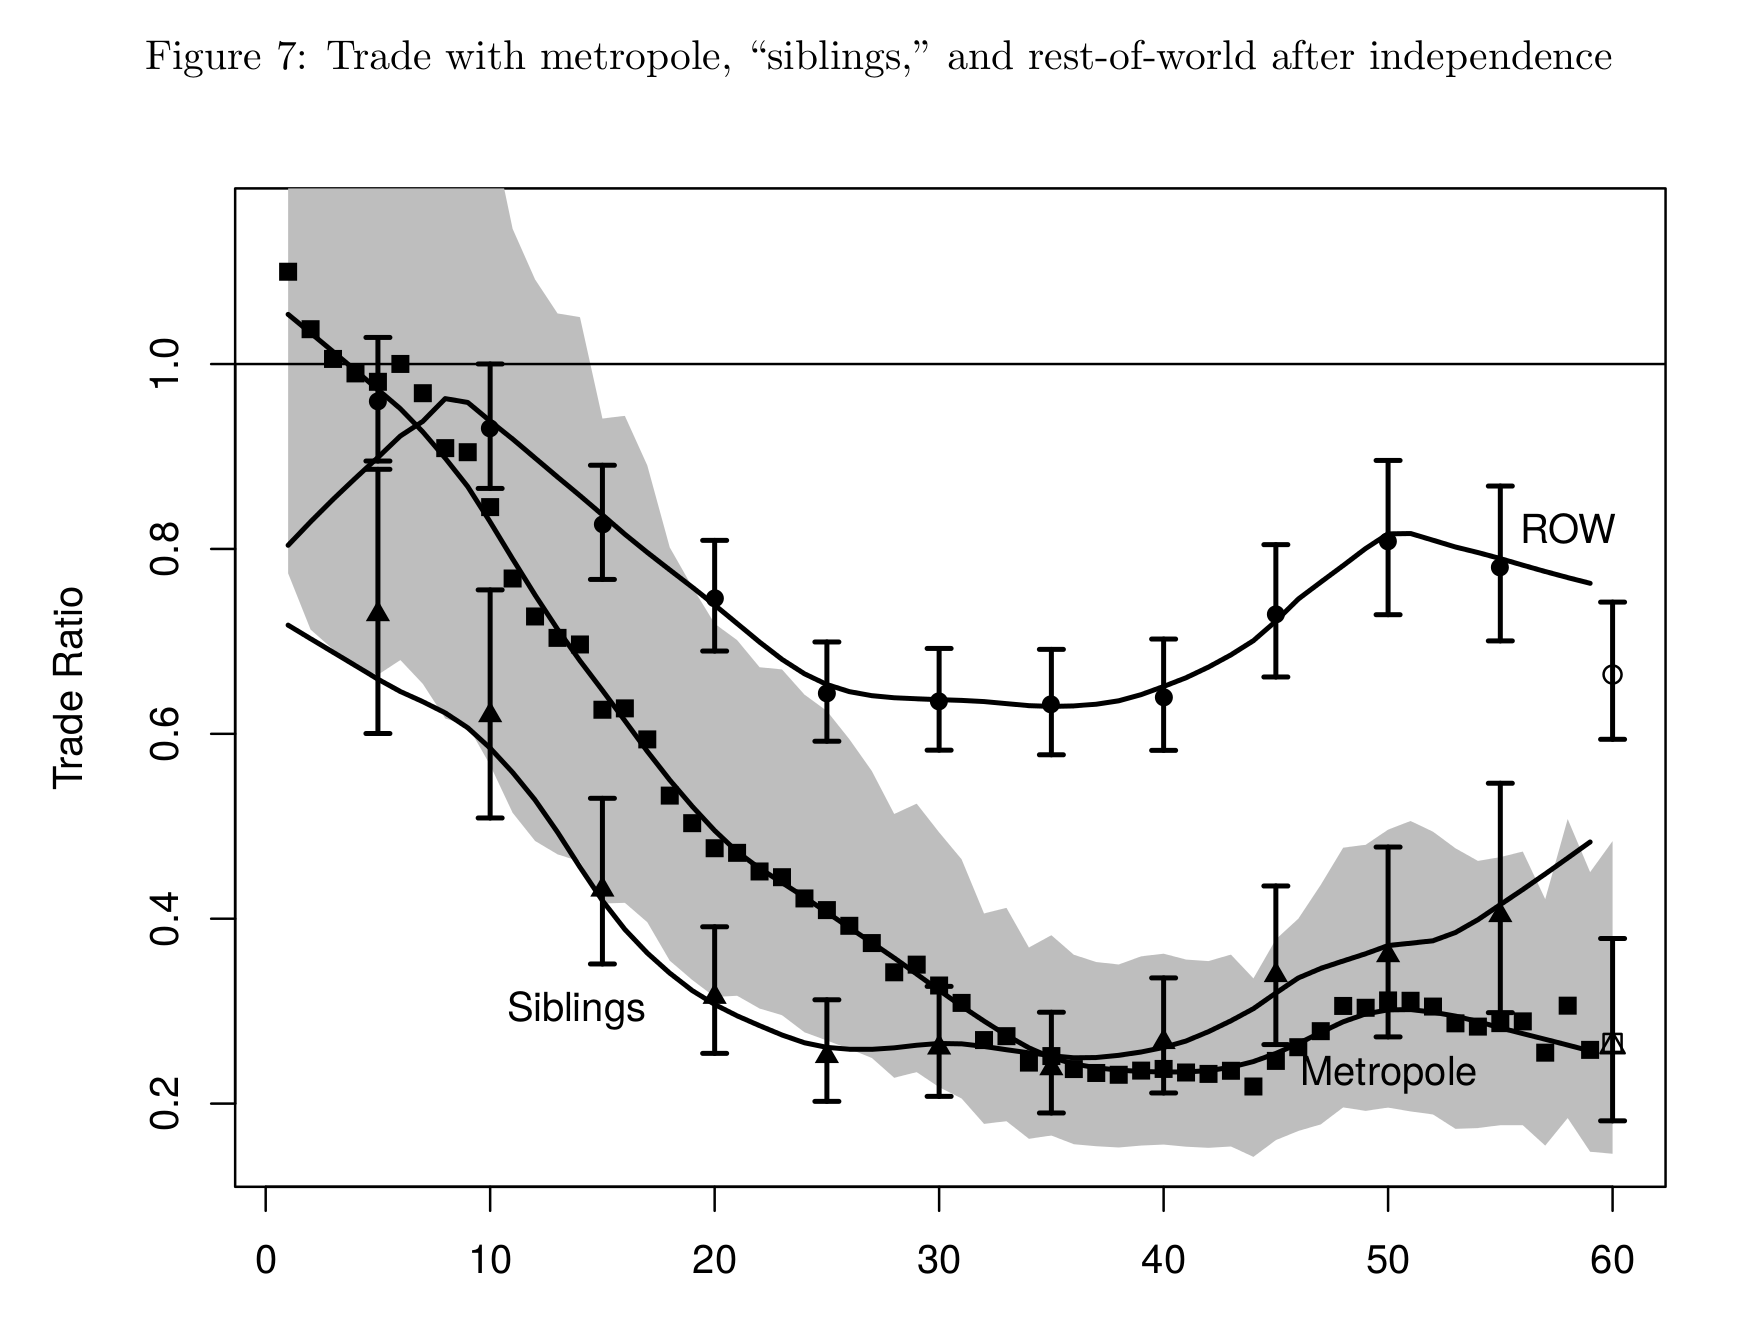
\includegraphics[scale=.7]{colonial_ties}
  \end{figure}
\end{frame}
%--------------------------------------

%--------------------------------------
\begin{frame}
  This trade loss between metropole and former colony, and among former colonies of same metropole is somewhat puzzling given
  \begin{itemize}
    \item Common institutions
    \item Same language
    \item Substantial bilateral migration
  \end{itemize}
  \medskip
  Barriers to trade seem to be low. 
  But despite the decline, trade levels are still higher than predicted by gravity model
\end{frame}
%--------------------------------------

%--------------------------------------
\begin{frame}{Colonial ties: France}
\framesubtitle{source: Head and Mayer, 2013}
  \begin{figure}
    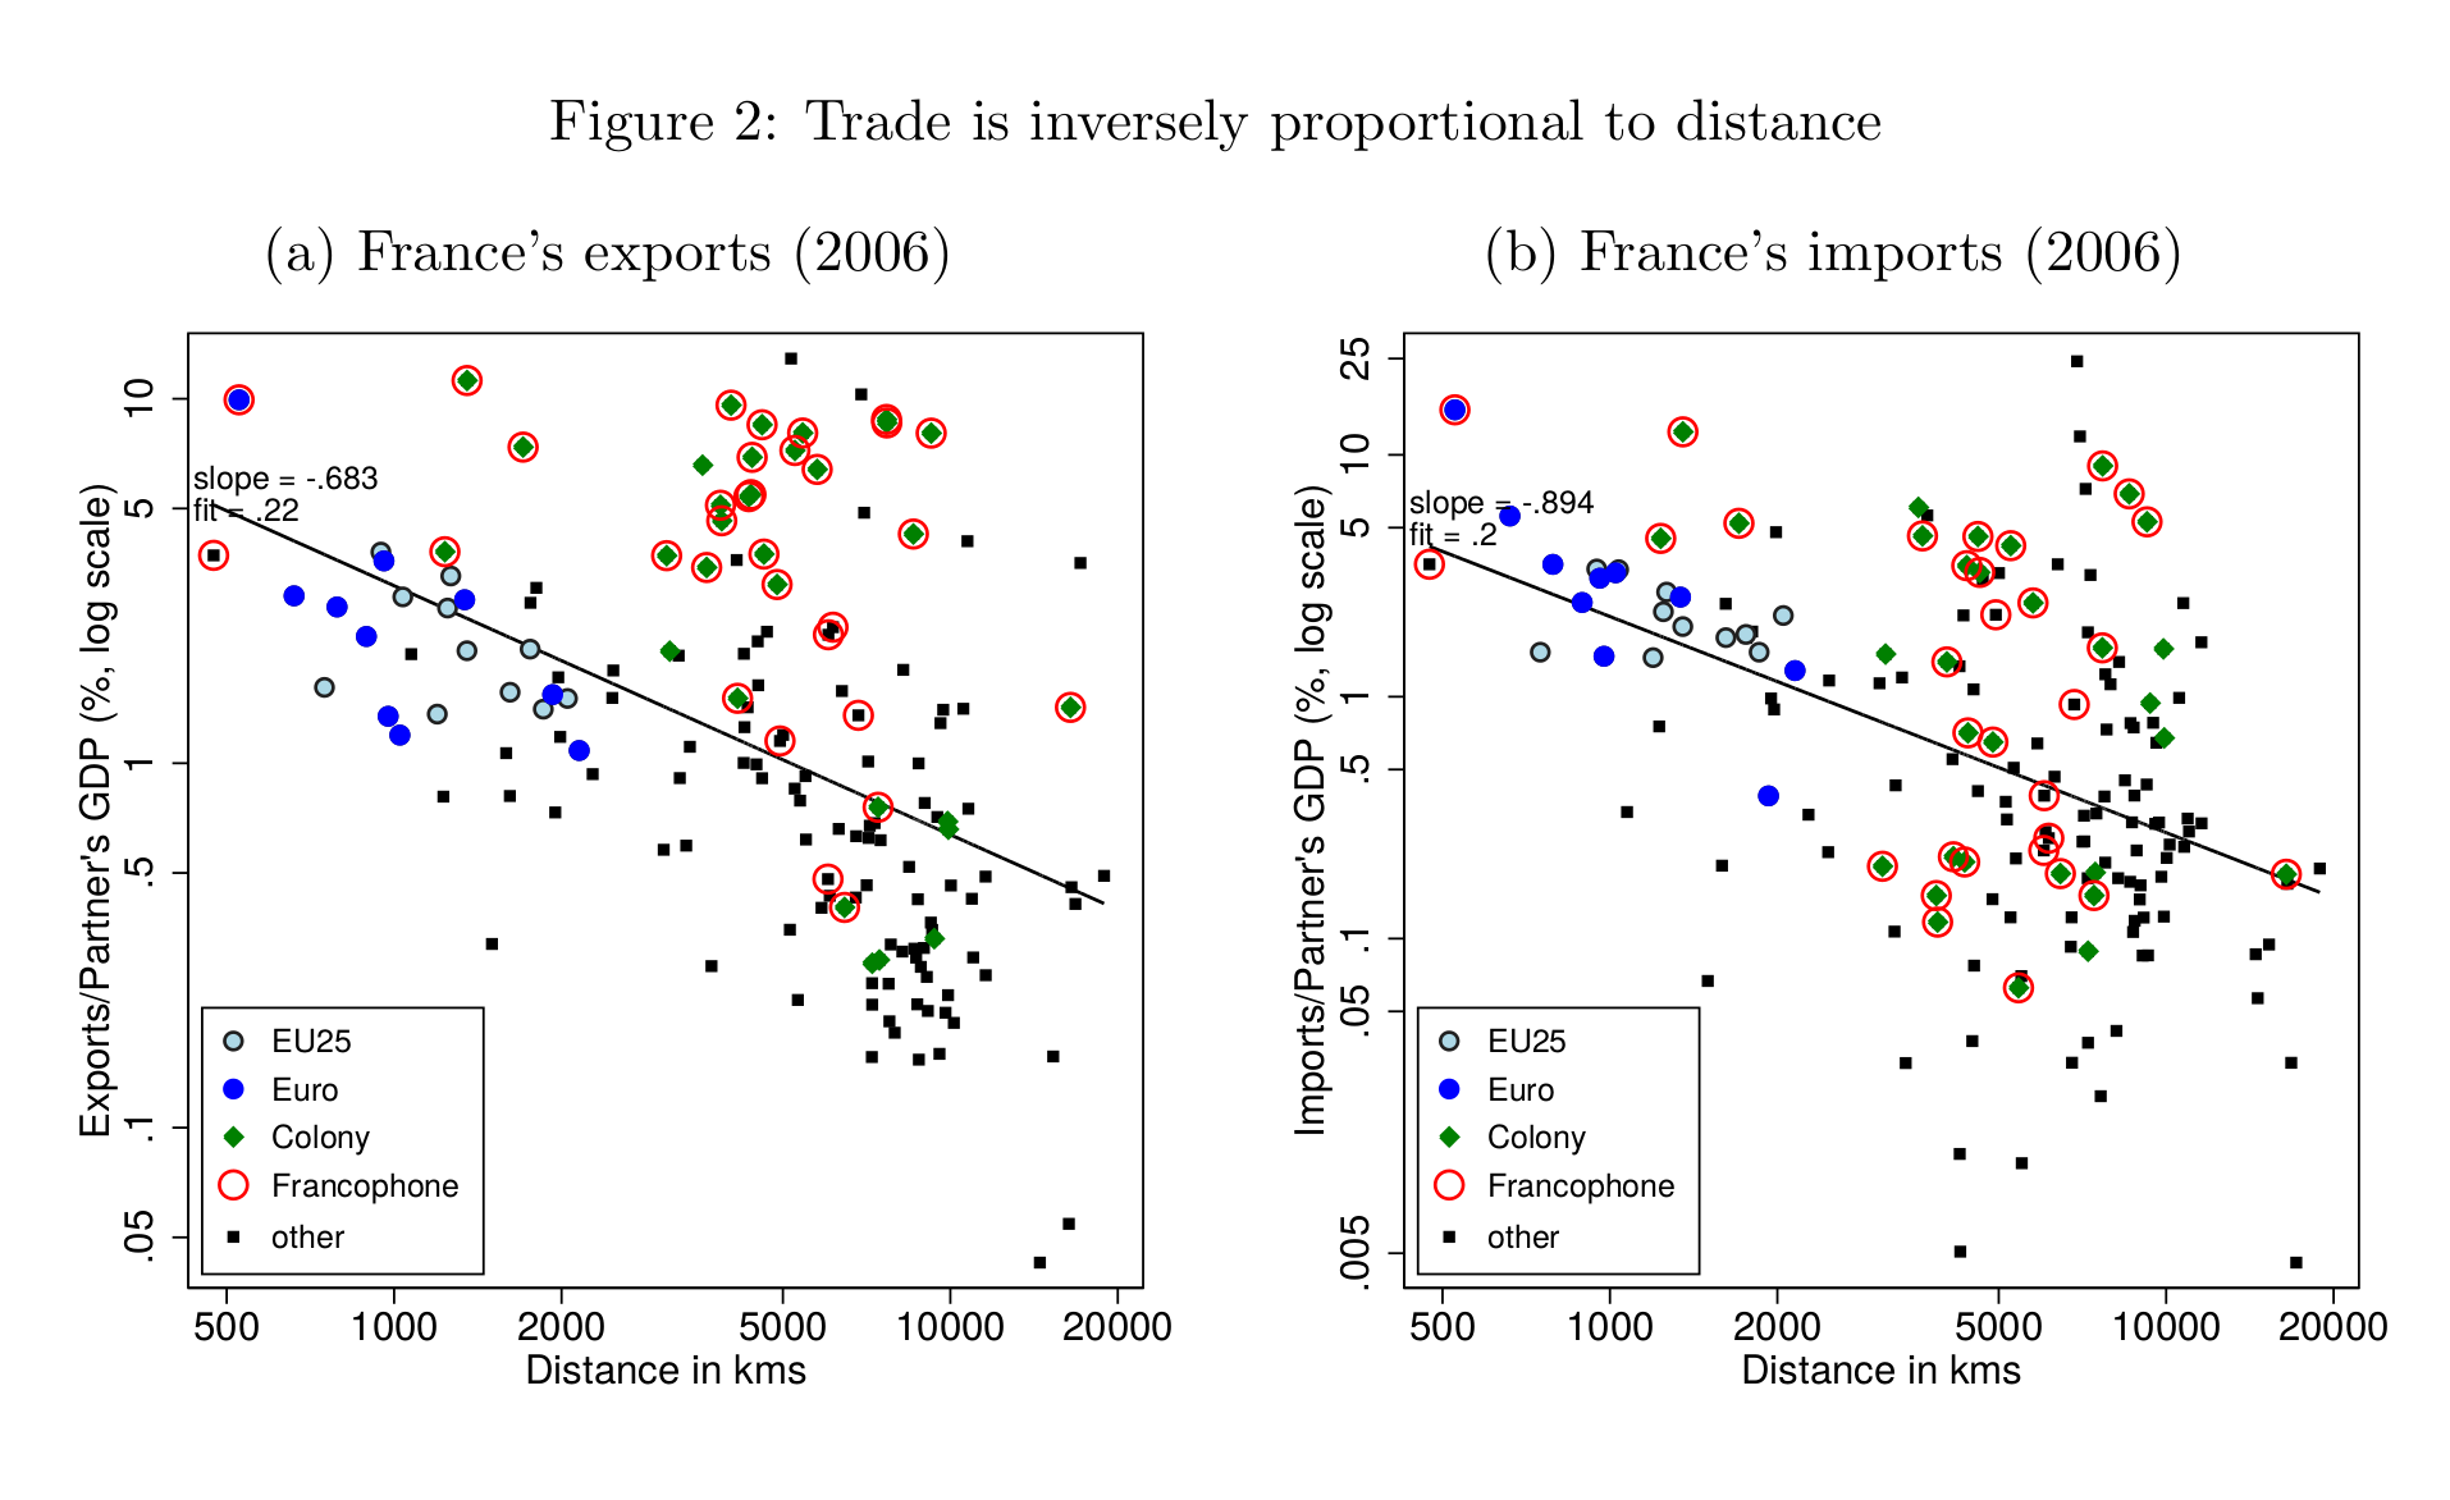
\includegraphics[scale=.5]{head_mayer3}
  \end{figure}
\end{frame}
%--------------------------------------

%------------------------------------------------------------------------------
\end{document}
